% ============================================================================
%  บทที่ 3: สถาปัตยกรรมและการออกแบบระบบ
% ============================================================================

\chapter{สถาปัตยกรรมและการออกแบบระบบ}
\label{ch:design}

% ============================================================================
\section{สถาปัตยกรรมระบบภาพรวม}
\label{sec:system_arch}
% ============================================================================

ระบบ Circular Pick and Place Robot ออกแบบตามหลัก Cyber-Physical System
โดยแบ่งสถาปัตยกรรมออกเป็น Physical Layer ซึ่งประกอบด้วยฮาร์ดแวร์จริง
และ Cyber Layer ซึ่งประกอบด้วยโครงสร้าง Firmware และ Communication
ภายใน STM32G474RE ดังแสดงใน\cref{fig:sys_arch}

% -----------------------------------------------------------------------
% รูปที่: System Architecture Overview
% ชื่อไฟล์แนะนำ: fig_system_architecture.png
% เนื้อหา: Layered block diagram แสดง 4 ระดับ (External $\rightarrow$ STM32 Cyber $\rightarrow$
%          Power Management $\rightarrow$ Physical Actuators/Sensors)
%          พร้อม color coding: blue=signal, red=power, green=mechanical
% -----------------------------------------------------------------------
\begin{figure}[H]
    \centering
    
\includegraphics[width=0.95\textwidth]{fig_system_architecture}
    \caption{System Architecture ของระบบ Circular Pick and Place Robot
             แสดง Physical Architecture และ Cyber Architecture}
    \label{fig:sys_arch}
\end{figure}

% -----------------------------------------------------------------------
\subsection{ห่วงโซ่การส่งกำลัง (Power Transmission Chain)}
\label{subsec:drivetrain_arch}
% -----------------------------------------------------------------------

ข้อกำหนด P3 กำหนดให้ความเร็วเชิงมุมที่เพลาแขนกลอยู่ในช่วง
$2.9 \leq \omega \leq 5.84$\,rad/s และ P4 กำหนดให้ความเร่งสูงสุด
$\alpha_{max} \leq 22.0$\,rad/s$^2$ ในขณะที่มอเตอร์ RS-775 มีความเร็วสูงสุด
5,950\,RPM ($\approx 623$\,rad/s) แสดงว่าระบบต้องการอัตราทดรวม
ในช่วง $N \approx 70$ เพื่อแปลงความเร็วสูงของมอเตอร์ให้เป็น
แรงบิดสูงสำหรับงานหยิบวางชิ้นงาน 2\,kg ที่รัศมี 500\,mm

การบรรลุอัตราทดดังกล่าวด้วย Single-stage Gearbox เพียงอย่างเดียว
จะทำให้ขนาดของ Gearbox ใหญ่เกินขีดจำกัดฐาน 200$\times$200\,mm
(ข้อกำหนด M1) ระบบจึงออกแบบเป็น 2-stage โดยแยกหน้าที่ดังนี้

\begin{itemize}
  \item \textbf{Planetary Gearbox} ($N_g = 24$): รับภาระ Torque Amplification
        หลัก เนื่องจาก Planetary configuration ให้อัตราทดสูงในขนาด
        Footprint เล็กกว่า Spur Gear ที่อัตราทดเทียบเท่า
  \item \textbf{Belt Drive HTD5M} ($N_b = 70/24 \approx 2.917$):
        ทำหน้าที่ปรับ Layout โดยส่งกำลังข้ามระยะ Center Distance 181.25\,mm
        เพื่อแยกตำแหน่งมอเตอร์ออกจากจุดหมุนของแขนกล
        ซึ่งช่วยลดโมเมนต์ความเฉื่อยของส่วนที่หมุน
        และยังทำให้สามารถติดตั้ง Encoder ได้โดยตรง
        ที่ Output Shaft โดยไม่ผ่าน Gearbox
\end{itemize}

อัตราทดรวม $N = N_g \times N_b = 24 \times 2.917 = 70$ และ
ประสิทธิภาพรวม $\eta = \eta_{gear} \times \eta_{belt} = 0.88 \times 0.95 = 0.836$
ให้แรงบิดที่เพลาแขนกล

\begin{equation}
  T_{arm} = T_{motor} \times N \times \eta
           = 0.0955 \times 70 \times 0.836
           = 5.40\,\text{N}\cdot\text{m}
  \label{eq:tarm_verify}
\end{equation}

ซึ่งมี Safety Factor เทียบกับแรงบิดที่ต้องการ
$T_{req} = J \cdot \alpha_{min} \times SF = 0.5764 \times 2.0 \times 2.0 = 2.31$\,N$\cdot$m
คือ $SF_{actual} = 5.40 / 2.31 = 2.34 > 2.0$ \textbf{(ผ่าน P3, P4)}

\textbf{การติดตั้ง Encoder ที่ Output Shaft:}
เพื่อลด Backlash Error ที่สะสมจากทั้ง Planetary Gearbox และ Belt Drive
Encoder AMT-103 จึงติดตั้งโดยตรงที่ Output Shaft ซึ่งเป็นตำแหน่ง
\emph{หลัง} ระบบส่งกำลังทั้งหมด Control Loop จึงปิดผ่านตำแหน่ง
จริงของแขนกลโดยตรง ทำให้ Backlash ในทุก Stage
ไม่ส่งผลต่อ Closed-loop Accuracy และ Repeatability (A2)

% -----------------------------------------------------------------------
% รูปที่: แผนผังห่วงโซ่การส่งกำลัง
% ชื่อไฟล์แนะนำ: fig_drivetrain_chain.png
% เนื้อหา: Block diagram ลำดับ Motor $\rightarrow$ Planetary Gearbox $\rightarrow$ Belt $\rightarrow$ Output Shaft
%          แสดงค่า RPM, Torque, และ N ที่แต่ละจุด พร้อมตำแหน่ง Encoder
% -----------------------------------------------------------------------
\begin{figure}[H]
    \centering
    
\includegraphics[width=\textwidth]{fig_drivetrain_chain}
    \caption{แผนผังห่วงโซ่การส่งกำลังแสดงการเปลี่ยนแปลงความเร็วและแรงบิด
             ตั้งแต่มอเตอร์ถึงแขนกล พร้อมตำแหน่ง Encoder ที่ Output Shaft}
    \label{fig:drivetrain_chain}
\end{figure}

% -----------------------------------------------------------------------
\subsection{Application Finite State Machine}
\label{subsec:fsm_arch}
% -----------------------------------------------------------------------

โครงสร้าง FSM ออกแบบให้ตอบสนองข้อกำหนดด้านความปลอดภัยและการใช้งาน
พร้อมกันในเวลาเดียว ระบบมี 5 สถานะหลักดังนี้

\begin{itemize}
  \item \textbf{\texttt{INIT}:} ตรวจสอบฮาร์ดแวร์และโหลดค่า Configuration
        จาก Flash ก่อนอนุญาตให้ระบบทำงาน
  \item \textbf{\texttt{HOMING}:} ค้นหาจุด Home ด้วย Two-Stage Homing
        (Coarse Search ไป Fine Search ด้วย Proximity Sensor)
        ตามข้อกำหนด A3 ที่ต้องสามารถตั้งจุด Home ได้หลังติดตั้ง
  \item \textbf{\texttt{IDLE}:} พร้อมรับคำสั่ง รอ Command จาก Modbus
        หรือ Joystick โดยตรวจสอบ Heartbeat Watchdog ต่อเนื่อง
  \item \textbf{\texttt{RUNNING}:} กำลังประมวลผล Motion Sequence
        ทั้ง Pick-Place Cycle และ Manual Jog
  \item \textbf{\texttt{FAULT}:} หยุดฉุกเฉิน ตัด PWM ทันที
        และ Log Fault Code เพื่อ Diagnosis
\end{itemize}

ทุกสถานะสามารถเข้าสู่ \texttt{FAULT} ได้จาก E-Stop Hardware หรือ
Software Safety Fault (Overcurrent, Heartbeat Timeout, Workspace Violation)
โดยไม่ผ่านสถานะกลาง เพื่อรับประกัน Worst-case Response Time
ที่ขึ้นกับ TIM6 ISR Period ($\leq 1$\,ms) เท่านั้น

สถานะ \texttt{FAULT} ตัดเฉพาะ PWM Output (Motor Power)
แต่ STM32 ยังคงรัน Firmware ต่อเนื่องเพื่อรับ Reset Command
และรายงาน Fault Code ผ่าน Modbus ซึ่งเป็นไปตามข้อกำหนด E6
ที่กำหนดให้ Controller มีไฟเลี้ยงแม้หลังกด E-Stop
สอดคล้องกับการออกแบบ Power Bus แบบ Dual-rail ใน\cref{subsec:elec_arch}

% -----------------------------------------------------------------------
% รูปที่: FSM State Diagram
% ชื่อไฟล์แนะนำ: fig_fsm_diagram.png
% เนื้อหา: State diagram แสดง 5 states (INIT, HOMING, IDLE, RUNNING, FAULT)
%          พร้อม transition conditions และ entry/exit actions
%          เน้น FAULT transitions จากทุก state ด้วยลูกศรสีแดง
% -----------------------------------------------------------------------
\begin{figure}[H]
    \centering
    
\includegraphics[width=0.80\textwidth]{fig_fsm_diagram}
    \caption{Application FSM แสดง 5 สถานะหลักและเงื่อนไข Transition
             โดย FAULT สามารถถูก Trigger ได้จากทุกสถานะ (ลูกศรสีแดง)}
    \label{fig:fsm_diagram}
\end{figure}

% ============================================================================
\section{การออกแบบเชิงกล}
\label{sec:mech_design}
% ============================================================================

\subsection{สถาปัตยกรรมเชิงกลโดยรวม}
\label{subsec:mech_arch}

โครงสร้างเชิงกลของระบบแบ่งออกเป็น 3 ส่วนหลักที่ประกอบกัน ได้แก่
ส่วนฐาน (Base) ที่ยึดกับแท่นของลูกค้าด้วยสกรู M8 ตามข้อกำหนด M7,
ส่วนแขนกล (Rotating Arm) รัศมี 500\,mm ที่หมุนรอบแกนแนวตั้ง
และชุดส่งกำลัง 2-stage ที่อธิบายใน\cref{subsec:drivetrain_arch}
ภาพรวม CAD Assembly แสดงใน\cref{fig:mech_cad}

% -----------------------------------------------------------------------
% รูปที่: CAD Assembly ภาพรวม
% ชื่อไฟล์แนะนำ: fig_cad_assembly.png
% เนื้อหา: CAD render มุมมอง Isometric แสดง Base, Arm, Gearbox,
%          Belt Drive, Encoder mount และ Gripper Housing
%          ควร label ส่วนประกอบหลักด้วย callout
% -----------------------------------------------------------------------
\begin{figure}[H]
    \centering
    
\includegraphics[width=0.75\textwidth]{fig_cad_assembly}
    \caption{CAD Assembly ของระบบเชิงกล แสดงส่วนประกอบหลักทั้งหมด}
    \label{fig:mech_cad}
\end{figure}

% -----------------------------------------------------------------------
\subsection{การคำนวณเพลา}
\label{subsec:shaft_calc}
% -----------------------------------------------------------------------

การคำนวณขนาดเพลาดำเนินการตาม Maximum Shear Stress Theory (ASME Code)
โดยมีจุดวิกฤตอยู่ที่ตำแหน่งลูกปืนบน ซึ่งรับทั้งโมเมนต์ดัดจากน้ำหนัก
ปลายแขนและแรงดึงสายพานพร้อมกัน

\subsubsection{พารามิเตอร์และวัสดุ}

\begin{table}[H]
  \centering
  \caption{พารามิเตอร์ภาระโหลดของระบบเพลา}
  \label{tab:shaft_loads}
  \begin{tabular}{llll}
    \toprule
    พารามิเตอร์ & สัญลักษณ์ & ค่า & หน่วย \\
    \midrule
    มวลโหลดที่ปลายเพลา        & $m$        & 3.72   & kg \\
    น้ำหนักโหลดในแนวดิ่ง       & $W$        & 37.20  & N \\
    ระยะเยื้องศูนย์            & $L_{cg}$   & 46.63  & mm \\
    ความเร็วรอบ               & $n$        & 85.00  & RPM \\
    แรงเหวี่ยงหนีศูนย์กลาง     & $F_c$      & 13.75  & N \\
    แรงดึงสายพานรวม            & $F_{belt}$ & 130.00 & N \\
    ระยะจากโหลดถึงลูกปืนบน    & $L_1$      & 25.25  & mm \\
    ระยะลูกปืนบนถึงล่าง        & $L_2$      & 37.25  & mm \\
    \bottomrule
  \end{tabular}
\end{table}

วัสดุเพลาเลือกใช้ Stainless Steel AISI~304
เนื่องจากเป็นวัสดุมาตรฐานที่หาซื้อได้ง่ายในตลาดไทย
มี Yield Strength $S_{yt} = 215$\,MPa
เพียงพอสำหรับการรับภาระในระบบนี้
และ Allowable Shear Stress ตามมาตรฐาน ASME คือ

\begin{equation}
  \tau_{allow} = 0.30 \times S_{yt} = 0.30 \times 215 = 64.5\,\text{MPa}
  \label{eq:shaft_tau_allow}
\end{equation}

% -----------------------------------------------------------------------
% รูปที่: Free Body Diagram เพลา
% ชื่อไฟล์แนะนำ: fig_shaft_fbd.png
% เนื้อหา: FBD แสดง W, Fc, Fbelt ที่กระทำต่อเพลา
%          พร้อม reaction forces ที่ลูกปืนบนและล่าง
%          และระบุจุดวิกฤตด้วยลูกศรหรือ highlight
% -----------------------------------------------------------------------
\begin{figure}[H]
    \centering
    
\includegraphics[width=0.75\textwidth]{fig_shaft_fbd}
    \caption{Free Body Diagram ของระบบเพลาแสดงแรงและโมเมนต์ที่จุดวิกฤต}
    \label{fig:shaft_fbd}
\end{figure}

\subsubsection{การวิเคราะห์โมเมนต์ดัด}

โมเมนต์ดัดจากโหลดปลายแขนและแรงเหวี่ยง

\begin{equation}
  M_{overhang} = (W + F_c) \times L_1
               = (37.20 + 13.75) \times 0.02525
               = 1.287\,\text{N}\cdot\text{m}
  \label{eq:shaft_m_overhang}
\end{equation}

โมเมนต์ดัดจากแรงดึงสายพาน

\begin{equation}
  M_{belt} = F_{belt} \times L_1
           = 130.00 \times 0.02525
           = 3.283\,\text{N}\cdot\text{m}
  \label{eq:shaft_m_belt}
\end{equation}

โมเมนต์รวม Worst-case โดย Vector Superposition (ทิศทางเสริมกัน)

\begin{equation}
  M_{total} = 5.014\,\text{N}\cdot\text{m}
  \label{eq:shaft_m_total}
\end{equation}

\subsubsection{การคำนวณขนาดเพลา}

เลือก Fatigue Shock Factors $C_m = 2.0$ (Bending) และ $C_t = 1.5$ (Torsion)
สำหรับสภาวะ Light Shock เนื่องจาก S-curve Trajectory จำกัด Jerk
ให้ไม่เกิน $j_{max} = 1400$\,rad/s$^3$ ทำให้ภาระที่เพลา
เปลี่ยนแปลงแบบต่อเนื่องไม่ใช่ Impact Load
แต่ยังคง $C_m > 1$ เพื่อรองรับ Transient ที่อาจเกิดขณะ
Emergency Stop

\begin{equation}
  d_{min} = \left[
    \frac{16}{\pi\,\tau_{allow}}
    \sqrt{(C_m M_{total})^2 + (C_t T)^2}
  \right]^{1/3}
  \label{eq:shaft_dmin}
\end{equation}

\begin{equation}
  d_{min} = \left[
    \frac{16}{\pi \times 64.5 \times 10^6}
    \sqrt{(2.0 \times 5.014)^2 + (1.5 \times 5.398)^2}
  \right]^{1/3}
  = 10.59\,\text{mm}
  \label{eq:shaft_result}
\end{equation}

\subsubsection{การออกแบบ Step Shaft}

แม้ว่า $d_{min} = 10.59$\,mm จากการวิเคราะห์ความล้า
แต่ขนาดจริงที่จุดวิกฤตถูกกำหนดโดย Bearing Seat ของ
SKF~30203 Tapered Roller Bearing ซึ่งมี ID~=~17\,mm
ดังนั้นจึงเลือก $d_{actual} = 17$\,mm ที่จุดวิกฤต
ซึ่งให้ FOS~$\geq 1.6$ เทียบกับ $d_{min}$

เพลาออกแบบเป็น Step Shaft เพื่อรองรับ Bearing
ที่ขนาดต่างกัน และสร้าง Shoulder สำหรับ Axial Location
ดังสรุปใน\cref{tab:shaft_summary}

\begin{table}[H]
  \centering
  \caption{สรุปผลการคำนวณเพลาและการออกแบบ Step Shaft}
  \label{tab:shaft_summary}
  \begin{tabular}{lccl}
    \toprule
    พารามิเตอร์ & ค่า & หน่วย & หมายเหตุ \\
    \midrule
    $M_{total}$ (Worst-case)  & 5.014 & N$\cdot$m & Vector Superposition \\
    $T$ (Torsion)             & 5.398 & N$\cdot$m & จากระบบส่งกำลัง \\
    $d_{min}$ (คำนวณ)         & 10.59 & mm        & จุดวิกฤต (Fatigue) \\
    $d_{actual}$ (จุดวิกฤต)   & 17    & mm        & Bearing Seat SKF 30203 \\
    $d$ (ช่วงกลาง)            & 12    & mm        & ผ่าน \\
    $d$ (ช่วงปลาย)            & 8--10 & mm        & ไม่ใช่จุดวิกฤต \\
    \bottomrule
  \end{tabular}
\end{table}

% -----------------------------------------------------------------------
\subsection{การวิเคราะห์เพลาด้วย FEA (Shaft FEA)}
\label{subsec:shaft_fea}
% -----------------------------------------------------------------------

เพื่อยืนยันผลการคำนวณเชิงวิเคราะห์ใน\cref{subsec:shaft_calc}
ดำเนินการวิเคราะห์ Finite Element Analysis (Static Study)
ด้วย SOLIDWORKS Simulation โดยจำลองเพลาเป็น Beam Element
ซึ่งเหมาะสมกับโครงสร้างที่มี Aspect Ratio สูง (ความยาวรวม $\approx 68$\,mm
เทียบกับเส้นผ่าศูนย์กลางสูงสุด 17\,mm)
การใช้ Beam Mesh แทน Solid Mesh ในกรณีนี้ให้ความแม่นยำเทียบเท่า
แต่ใช้ Computational Cost ต่ำกว่าอย่างมีนัยสำคัญ
เนื่องจากทฤษฎี Euler–Bernoulli Beam ถูกต้องเมื่อ
$L/d > 10$ ซึ่งเป็นเงื่อนไขที่เพลานี้ตอบสนองได้

\subsubsection{สภาวะการจำลอง (FEA Setup)}

โมเดลเพลาแบบ Step Shaft สร้างขึ้นใน SOLIDWORKS โดยแบ่งออกเป็น
6 Beam Segment ตามขนาดเส้นผ่าศูนย์กลางที่เปลี่ยนไปในแต่ละช่วง
วัสดุที่ใช้คือ Stainless Steel AISI~304 ซึ่งสอดคล้องกับการออกแบบ
ใน\cref{subsec:shaft_calc}

\begin{table}[H]
  \centering
  \caption{คุณสมบัติวัสดุที่ใช้ใน FEA เพลา (AISI 304)}
  \label{tab:shaft_fea_material}
  \begin{tabular}{lll}
    \toprule
    คุณสมบัติ & ค่า & หน่วย \\
    \midrule
    Yield Strength   & $2.068 \times 10^8$ & N/m$^2$ \\
    Tensile Strength & $5.170 \times 10^8$ & N/m$^2$ \\
    Elastic Modulus  & $1.900 \times 10^{11}$ & N/m$^2$ \\
    Poisson's Ratio  & 0.29 & -- \\
    Mass Density     & 8,000 & kg/m$^3$ \\
    Shear Modulus    & $7.500 \times 10^{10}$ & N/m$^2$ \\
    \bottomrule
  \end{tabular}
\end{table}

กำหนด Boundary Conditions ดังนี้

\begin{itemize}
  \item \textbf{Fixture:} Immovable (No Translation) ที่ Joint
        ตำแหน่งลูกปืนบน (SKF~30203) และลูกปืนล่าง (F6901ZZ)
        จำลองการยึดแน่นของ Bearing Housing ในแนวรัศมี
  \item \textbf{Load:} แรงดึงสายพาน $F_{belt} = 130$\,N
        ในแนวรัศมีที่ตำแหน่ง Belt Pulley
        และ Moment $M = 1.7$\,N$\cdot$m
        (แรงบิดที่ส่งผ่านสายพานเมื่อระบบทำงานเต็มกำลัง)
  \item \textbf{Mesh:} Beam Mesh, 37 Nodes, 30 Elements
        (Automatic, High Quality)
\end{itemize}

% -----------------------------------------------------------------------
% รูปที่: Shaft FEA — Load and Fixture Setup
% ชื่อไฟล์แนะนำ: fig_shaft_fea_setup.png
% เนื้อหา: SOLIDWORKS screenshot แสดง Step Shaft พร้อม
%          Fixture ที่ตำแหน่งลูกปืน (สีฟ้า) และ
%          แรง F=130N + Moment=1.7N.m ที่ตำแหน่ง Pulley (ลูกศรสีชมพู)
% -----------------------------------------------------------------------
\begin{figure}[H]
    \centering
    
\includegraphics[width=0.75\textwidth]{fig_shaft_fea_setup}
    \caption{การตั้งค่าโมเดล FEA เพลา แสดง Fixture ที่ตำแหน่งลูกปืน
             และภาระแรงดึงสายพาน 130\,N พร้อม Moment 1.7\,N$\cdot$m}
    \label{fig:shaft_fea_setup}
\end{figure}

\subsubsection{ผลการวิเคราะห์ FEA เพลา}

% -----------------------------------------------------------------------
% รูปที่: Shaft FEA — Stress Distribution
% ชื่อไฟล์แนะนำ: fig_shaft_fea_stress.png
% เนื้อหา: SOLIDWORKS color map (Upper bound axial and bending stress)
%          Max = 2.221e+07 N/m² ที่ Element 24 (บริเวณ Belt Pulley seat)
%          แสดง deformed shape + color scale
% -----------------------------------------------------------------------
\begin{figure}[H]
    \centering
    
\includegraphics[width=0.75\textwidth]{fig_shaft_fea_stress}
    \caption{ผล FEA เพลา: การกระจายตัวของ Upper Bound Axial and Bending Stress
             (Max $= 2.221 \times 10^7$\,N/m$^2$ บริเวณตำแหน่ง Belt Pulley)}
    \label{fig:shaft_fea_stress}
\end{figure}

% -----------------------------------------------------------------------
% รูปที่: Shaft FEA — Displacement
% ชื่อไฟล์แนะนำ: fig_shaft_fea_displacement.png
% เนื้อหา: SOLIDWORKS color map ของ URES Resultant Displacement
%          Max = 4.721e-03 mm ที่ Node 30 (ปลายเพลาด้านล่าง)
% -----------------------------------------------------------------------
\begin{figure}[H]
    \centering
    
\includegraphics[width=0.75\textwidth]{fig_shaft_fea_displacement}
    \caption{ผล FEA เพลา: ระยะการเบี่ยงเบน (URES Displacement)
             (Max $= 4.721 \times 10^{-3}$\,mm ที่ปลายเพลา)}
    \label{fig:shaft_fea_displacement}
\end{figure}

% -----------------------------------------------------------------------
% รูปที่: Shaft FEA — Factor of Safety
% ชื่อไฟล์แนะนำ: fig_shaft_fea_fos.png
% เนื้อหา: SOLIDWORKS FOS color map
%          Min FOS = 9.313 ที่ Node 5 (บริเวณ Belt Pulley)
%          แสดง scale ด้านขวา พร้อม label Min FOS
% -----------------------------------------------------------------------
\begin{figure}[H]
    \centering
    
\includegraphics[width=0.75\textwidth]{fig_shaft_fea_fos}
    \caption{ผล FEA เพลา: ค่าความปลอดภัย (Factor of Safety)
             (Min FOS $= 9.313$ บริเวณตำแหน่ง Belt Pulley)}
    \label{fig:shaft_fea_fos}
\end{figure}

% -----------------------------------------------------------------------
% รูปที่: Shaft FEA — Shear Force Diagram
% ชื่อไฟล์แนะนำ: fig_shaft_fea_shear.png
% เนื้อหา: SOLIDWORKS Shear Force in Dir2 diagram
%          แสดง shear diagram ตามความยาวเพลา
%          Max shear = 88.12 N ในช่วง Belt Pulley
% -----------------------------------------------------------------------
\begin{figure}[H]
    \centering
    
\includegraphics[width=0.75\textwidth]{fig_shaft_fea_shear}
    \caption{ผล FEA เพลา: แผนภาพแรงเฉือน (Shear Force in Dir2)
             แสดงการเปลี่ยนแปลงแรงเฉือนตลอดความยาวเพลา}
    \label{fig:shaft_fea_shear}
\end{figure}

% -----------------------------------------------------------------------
% รูปที่: Shaft FEA — Bending Moment Diagram
% ชื่อไฟล์แนะนำ: fig_shaft_fea_moment.png
% เนื้อหา: SOLIDWORKS Moment about Dir2 diagram
%          Max moment = 1.7 N.m ที่ Fixture ด้านบน
%          แสดง moment diagram ตามความยาวเพลา
% -----------------------------------------------------------------------
\begin{figure}[H]
    \centering
    
\includegraphics[width=0.75\textwidth]{fig_shaft_fea_moment}
    \caption{ผล FEA เพลา: แผนภาพโมเมนต์ดัด (Bending Moment about Dir2)
             แสดงการกระจาย Bending Moment ตลอดความยาวเพลา}
    \label{fig:shaft_fea_moment}
\end{figure}

\subsubsection{การตรวจสอบความสอดคล้องกับการคำนวณเชิงวิเคราะห์}

\begin{table}[H]
  \centering
  \caption{สรุปผลการวิเคราะห์ FEA เพลาเทียบกับการคำนวณ ASME Code}
  \label{tab:shaft_fea_results}
  \begin{tabular}{lcccc}
    \toprule
    พารามิเตอร์ & ผล FEA & เกณฑ์ & หน่วย & ผล \\
    \midrule
    Max Bending+Axial Stress & $2.221 \times 10^7$ & $< 2.068 \times 10^8$
      & N/m$^2$ & \textbf{ผ่าน} \\
    Max Displacement (URES)  & $4.721 \times 10^{-3}$ & --
      & mm & -- \\
    Min Factor of Safety     & 9.313 & $> 2.0$
      & -- & \textbf{ผ่าน} \\
    \bottomrule
  \end{tabular}
\end{table}

ผล FEA ยืนยันผลการคำนวณ ASME Code ใน\cref{subsec:shaft_calc}
โดย Min FOS = 9.313 สูงกว่าที่คำนวณได้จาก $d_{min} = 10.59$\,mm
เนื่องจากเส้นผ่าศูนย์กลางจริงที่จุดวิกฤต $d_{actual} = 17$\,mm
มี Margin สูงกว่าค่าขั้นต่ำอย่างมาก
Max Displacement เพียง $4.721 \times 10^{-3}$\,mm
บ่งชี้ว่าเพลามีความแข็งเกร็งเพียงพอ
และการโก่งตัวของเพลาจะไม่ส่งผลต่อ Alignment
ของ Encoder ที่ติดตั้งที่ Output Shaft
ซึ่งเป็นปัจจัยสำคัญต่อความแม่นยำของ Closed-loop Control (A1, A2)

% -----------------------------------------------------------------------
% รูปที่: Step Shaft Drawing
% ชื่อไฟล์แนะนำ: fig_shaft_drawing.png
% เนื้อหา: Engineering drawing แสดงขนาดแต่ละช่วง (17/12/8-10 mm)
%          ตำแหน่ง Bearing Seat, Key slot และ Shoulder
% -----------------------------------------------------------------------
\begin{figure}[H]
    \centering
    
\includegraphics[width=0.85\textwidth]{fig_shaft_drawing}
    \caption{Step Shaft Drawing แสดงขนาดเพลาแต่ละช่วงและตำแหน่งลูกปืน}
    \label{fig:shaft_drawing}
\end{figure}

% -----------------------------------------------------------------------
\subsection{การคำนวณสายพาน}
\label{subsec:belt_calc}
% -----------------------------------------------------------------------

ระบบเลือกใช้สายพาน HTD5M (High Torque Drive, 5\,mm Pitch)
แทน XL หรือ GT2 เนื่องจาก Curvilinear Tooth Profile ของ HTD
ออกแบบมาเฉพาะสำหรับ High Torque Low Speed Application
โดยกระจายแรงกดที่ฟันสายพานได้สม่ำเสมอกว่า Trapezoidal Profile
ของ XL ซึ่งมีความเสี่ยง Tooth Jump เมื่อ Tight Side Tension สูง

\subsubsection{ค่าเริ่มต้นของระบบสายพาน}

\begin{table}[H]
  \centering
  \caption{ค่าเริ่มต้นของระบบสายพาน HTD5M}
  \label{tab:belt_initial}
  \begin{tabular}{llll}
    \toprule
    พารามิเตอร์ & สัญลักษณ์ & ค่า & หน่วย \\
    \midrule
    ประเภทสายพาน    & --        & HTD5M (Steel Cord, Joined Endless) & -- \\
    ความกว้างสายพาน & $b_0$     & 15    & mm \\
    Belt Pitch      & $P_b$     & 5     & mm \\
    Driver Pulley   & $z_1$     & 24    & teeth \\
    Driven Pulley   & $z_2$     & 70    & teeth \\
    ระยะศูนย์กลาง   & $e$       & 181.25 & mm \\
    แรงบิดที่แขนกล  & $T_{arm}$ & 8.3279 & N$\cdot$m \\
    อัตราทด         & $i$       & 2.917 & -- \\
    \bottomrule
  \end{tabular}
\end{table}

\subsubsection{Peripheral Force}

\begin{equation}
  d_1 = \frac{z_1 P_b}{\pi} = \frac{24 \times 5}{\pi} = 38.20\,\text{mm}, \qquad
  d_2 = \frac{z_2 P_b}{\pi} = \frac{70 \times 5}{\pi} = 111.41\,\text{mm}
  \label{eq:belt_diameters}
\end{equation}

\begin{equation}
  F_U = \frac{2\,T_{driver}}{d_1}
      = \frac{2 \times 2.855}{0.03820}
      = 130\,\text{N}
  \label{eq:belt_fu}
\end{equation}

ค่า Admissible Peripheral Force ของ HTD5M ขนาด 15\,mm
จาก Habasit Catalog คือ 400\,N
ดังนั้น $F_U = 130\,\text{N} \ll 400\,\text{N}$ \textbf{(ผ่าน)}
ความกว้าง 15\,mm เกินค่าขั้นต่ำที่คำนวณได้ ($b_{req} = 3.9$\,mm)
อย่างมีนัยสำคัญ เพื่อรองรับ Misalignment ที่อาจเกิดขึ้นใน
การประกอบจริง และลดความเสี่ยง Edge Wear ของสายพาน

\begin{figure}[H]
    \centering
    
\includegraphics[width=0.5\textwidth]{fig_habasit_catalog}
    \caption{ตารางค่า Admissible Peripheral Force ของสายพาน HTD5M
             จาก Habasit Engineering Guide แสดงพิกัด 400\,N
             สำหรับความกว้าง 15\,mm}
    \label{fig:habasit_catalog}
\end{figure}


\subsubsection{Belt Length และ Teeth in Mesh}

\begin{equation}
  z_b = \frac{2e}{P_b} + \frac{z_1+z_2}{2}
      + \frac{P_b}{4e}\!\left(\frac{z_2-z_1}{\pi}\right)^2
      = 119\,\text{teeth}, \qquad
  l_0 = z_b \times P_b = 595\,\text{mm}
  \label{eq:belt_length}
\end{equation}

\begin{equation}
  z_m = z_1\!\left(0.5 - \frac{d_2-d_1}{2\pi e}\right)
      = 6.74\,\text{teeth} > 5
  \quad\Rightarrow\quad t_m = 1.0\;\textbf{(ผ่าน)}
  \label{eq:belt_zm}
\end{equation}

\subsubsection{Belt Tension และ Width Verification}

\begin{equation}
  F_1 = F_2 + F_U = 26 + 130 = 156\,\text{N (Tight Side)}, \qquad
  F_2 = 26\,\text{N (Slack Side)}
  \label{eq:belt_tension}
\end{equation}

\begin{table}[H]
  \centering
  \caption{สรุปผลการคำนวณสายพาน HTD5M}
  \label{tab:belt_summary}
  \begin{tabular}{lcccc}
    \toprule
    พารามิเตอร์ & ผลคำนวณ & เกณฑ์ & หน่วย & ผล \\
    \midrule
    Peripheral Force $F_U$ & 130  & $\leq 400$ & N     & \textbf{ผ่าน} \\
    Teeth in Mesh $z_m$    & 6.74 & $> 5$      & teeth & \textbf{ผ่าน} \\
    Belt Width $b_0$        & 15   & $\geq 3.9$ & mm    & \textbf{ผ่าน} \\
    Belt Length $l_0$       & 595  & --         & mm    & -- \\
    Tight Side Tension $F_1$ & 156 & --         & N     & -- \\
    Slack Side Tension $F_2$ & 26  & --         & N     & -- \\
    \bottomrule
  \end{tabular}
\end{table}

% -----------------------------------------------------------------------
\subsection{การเลือกตลับลูกปืนและการคำนวณอายุการใช้งาน}
\label{subsec:bearing_calc}
% -----------------------------------------------------------------------

เลือกตลับลูกปืน 2 ตำแหน่งโดยอ้างอิงมาตรฐาน ISO~281
ที่ความเร็วรอบ 85\,RPM

ลูกปืนบน (SKF~30203, Tapered Roller) เลือกเพราะต้องรับทั้ง
Radial Load จากแรงดึงสายพานและ Axial Load จากน้ำหนักแขนกล
พร้อมกัน ซึ่ง Tapered Roller Bearing รับ Combined Load
ได้ดีกว่า Deep Groove Ball Bearing ที่ขนาด Bore เดียวกัน
ลูกปืนล่าง (F6901ZZ, Deep Groove Ball) รับเฉพาะ
Radial Load เป็นหลักจึงเลือก Ball Bearing ที่มีแรงเสียดทานต่ำกว่า

\begin{table}[H]
  \centering
  \caption{ผลการคำนวณอายุการใช้งานของตลับลูกปืน}
  \label{tab:bearing_life}
  \begin{tabular}{lcccc}
    \toprule
    ตำแหน่ง / รุ่น & $C$ (kN) & $P$ (kN) & $L_{10h}$ (ชั่วโมง) & ผล \\
    \midrule
    SKF 30203 (Taper Roller, ลูกปืนบน)     & 23.400 & 0.2600
      & $6.1 \times 10^8$ & \textbf{ผ่าน} \\
    F6901ZZ (Deep Groove Ball, ลูกปืนล่าง) & 2.886  & 0.1388
      & $1.76 \times 10^6$ & \textbf{ผ่าน} \\
    \bottomrule
    \multicolumn{5}{l}{\small เกณฑ์มาตรฐานทั่วไปสำหรับเครื่องจักรกล:
      20,000--100,000 ชั่วโมง}\\
  \end{tabular}
\end{table}

\subsection{การวิเคราะห์การโก่งตัวด้วย FEA}
\label{subsec:fea}

ดำเนินการวิเคราะห์ Finite Element Analysis (Static Study)
ด้วย SOLIDWORKS Simulation ภายใต้โหลด 2\,kg ตามข้อกำหนด M3
วัสดุแขนกลเลือกใช้ Galvanized Steel แทน Stainless Steel AISI~304
เนื่องจากน้ำหนักที่เบากว่าช่วยลดโมเมนต์ความเฉื่อย $J$ ของส่วนที่หมุน
ซึ่งส่งผลโดยตรงต่อ Torque Budget และ Cycle Time (P1)
โดยยอมรับ Trade-off ด้าน Corrosion Resistance ที่ต่ำกว่า
เนื่องจากสภาพแวดล้อมการใช้งานเป็น Indoor Industrial

\subsubsection{สภาวะการจำลอง (FEA Setup)}

กำหนด Boundary Conditions ดังนี้

\begin{itemize}
  \item \textbf{Fixture:} Fixed Geometry ที่ขอบรูน็อตทั้งสองฝั่ง
        และหน้าสัมผัสที่แนบกับตัวฐานหุ่นยนต์
  \item \textbf{Load:} Remote Load 2.76\,kg ที่หน้าสัมผัสปลายแขน
        (ตำแหน่ง $x = -0.9$\,mm, $y = -46.82$\,mm, $z = 55.58$\,mm)
        โดยใช้ Remote Load แทน Point Load
        เพื่อกระจายแรงผ่าน Remote Point
        ตามน้ำหนักจริงของ Gripper และ Connection Rod รวมกัน
  \item \textbf{Mesh:} Solid, Blended Curvature-based,
        High Quality (Jacobian 16 Points),
        11,607 Nodes, 5,722 Elements
\end{itemize}

% -----------------------------------------------------------------------
% รูปที่: FEA Setup — Fixture และ Load Direction
% ชื่อไฟล์แนะนำ: fig_fea_setup_fixture.png
% เนื้อหา: SOLIDWORKS screenshot แสดงจุดจับยึด (สีฟ้า)
%          และทิศทางของภาระแรง (ลูกศรสีชมพู)
% -----------------------------------------------------------------------
\begin{figure}[H]
    \centering
    
\includegraphics[width=0.82\textwidth]{fig_fea_setup_fixture}
    \caption{โมเดลจำลอง FEA แสดงจุดจับยึด Fixture (สีฟ้า)
             และทิศทางของภาระแรง Remote Load (ลูกศรสีชมพู)}
    \label{fig:fea_setup_fixture}
\end{figure}

% -----------------------------------------------------------------------
% รูปที่: FEA Setup — Remote Load Parameters
% ชื่อไฟล์แนะนำ: fig_fea_setup_remoteload.png
% เนื้อหา: SOLIDWORKS screenshot แสดง Remote Mass = 2.76 kg
%          พร้อม coordinate ของ Remote Point
% -----------------------------------------------------------------------
\begin{figure}[H]
    \centering
    
\includegraphics[width=0.82\textwidth]{fig_fea_setup_remoteload}
    \caption{การตั้งค่า Remote Load 2.76\,kg แสดง Remote Point
             และ Moment of Inertia ที่กำหนด}
    \label{fig:fea_setup_remoteload}
\end{figure}

\subsubsection{การตรวจสอบเชิงวิเคราะห์ก่อน FEA (Analytical Verification)}

ก่อนดำเนินการ FEA ทำการตรวจสอบเบื้องต้นด้วยการคำนวณเชิงวิเคราะห์
โดยจำลองแขนกลเป็น Cantilever Beam หน้าตัด Galvanized Square Tube
$25 \times 25$\,mm หนา 1.4\,mm ความยาว $L = 0.5$\,m

Second Moment of Inertia ของหน้าตัดท่อสี่เหลี่ยม

\begin{equation}
  I = \frac{bh^3 - b_i h_i^3}{12}
    = \frac{25 \times 25^3 - 20.4 \times 20.4^3}{12}
    = 18{,}119.65\,\text{mm}^4
  \label{eq:arm_inertia}
\end{equation}

การโก่งตัวแบ่งออกเป็น 2 ส่วน ได้แก่
การโก่งจากน้ำหนักแขนกลเอง (Distributed Load $w$)
และการโก่งจากโหลดที่ปลายแขน (Point Load $P$)

\begin{align}
  \delta_1 &= \frac{wL^4}{8EI}
            = \frac{5.123 \times 0.5^4}
                   {8 \times 200{,}000 \times 18{,}119.65 \times 10^{-12}}
            = 0.0110\,\text{mm}
  \label{eq:deflection_dist} \\[6pt]
  \delta_2 &= \frac{PL^3}{3EI}
            = \frac{19.62 \times 0.5^3}
                   {3 \times 200{,}000 \times 18{,}119.65 \times 10^{-12}}
            = 0.2256\,\text{mm}
  \label{eq:deflection_point}
\end{align}

การโก่งตัวรวม

\begin{equation}
  \delta_{total} = \delta_1 + \delta_2
                = 0.0110 + 0.2256
                = 0.2366\,\text{mm} < 1.0\,\text{mm}
                \quad\textbf{(ผ่าน)}
  \label{eq:deflection_total}
\end{equation}

\subsubsection{ผลการวิเคราะห์ FEA}

\begin{table}[H]
  \centering
  \caption{คุณสมบัติวัสดุที่ใช้ใน FEA (Galvanized Steel)}
  \label{tab:fea_material}
  \begin{tabular}{lll}
    \toprule
    คุณสมบัติ & ค่า & หน่วย \\
    \midrule
    Yield Strength  & $2.35 \times 10^8$ & N/m$^2$ \\
    Elastic Modulus & $2.00 \times 10^{11}$ & N/m$^2$ \\
    Poisson's Ratio & 0.26 & -- \\
    Mass Density    & 7,850 & kg/m$^3$ \\
    \bottomrule
  \end{tabular}
\end{table}

% -----------------------------------------------------------------------
% รูปที่: Von Mises Stress Distribution
% ชื่อไฟล์แนะนำ: fig_fea_stress.png
% เนื้อหา: SOLIDWORKS color map ของ Von Mises Stress
%          Max = 2.721e+07 N/m² บริเวณขอบหน้าสัมผัสฐาน
%          ระบุจุด Max ด้วย callout
% -----------------------------------------------------------------------
\begin{figure}[H]
    \centering
    
\includegraphics[width=0.82\textwidth]{fig_fea_stress}
    \caption{ผล FEA: การกระจายตัวของ Von Mises Stress บนแขนกล
             (Max $= 2.721 \times 10^7$\,N/m$^2$ บริเวณขอบหน้าสัมผัสกับฐาน)}
    \label{fig:fea_stress}
\end{figure}

% -----------------------------------------------------------------------
% รูปที่: Displacement Distribution
% ชื่อไฟล์แนะนำ: fig_fea_displacement.png
% เนื้อหา: SOLIDWORKS color map ของ URES Displacement
%          Max = 2.337e-01 mm ที่ปลายแขนกล
% -----------------------------------------------------------------------
\begin{figure}[H]
    \centering
    
\includegraphics[width=0.82\textwidth]{fig_fea_displacement}
    \caption{ผล FEA: ระยะการแอ่นตัว (Displacement) บนแขนกล
             (Max $= 0.2337$\,mm ที่ปลายสุดของแขนกล)}
    \label{fig:fea_displacement}
\end{figure}

% -----------------------------------------------------------------------
% รูปที่: Factor of Safety Distribution
% ชื่อไฟล์แนะนำ: fig_fea_fos.png
% เนื้อหา: SOLIDWORKS color map ของ FOS
%          Min FOS = 8.6 ที่บริเวณขอบหน้าสัมผัสฐาน
% -----------------------------------------------------------------------
\begin{figure}[H]
    \centering
    
\includegraphics[width=0.82\textwidth]{fig_fea_fos}
    \caption{ผล FEA: ค่าความปลอดภัย (Factor of Safety)
             บนแขนกล (Min FOS $= 8.6$)}
    \label{fig:fea_fos}
\end{figure}

\begin{table}[H]
  \centering
  \caption{สรุปผลการวิเคราะห์ FEA เทียบกับข้อกำหนด M3}
  \label{tab:fea_results}
  \begin{tabular}{lcccc}
    \toprule
    พารามิเตอร์ & ผล FEA & เกณฑ์ & หน่วย & ผล \\
    \midrule
    Max Von Mises Stress & $2.721 \times 10^7$ & $< 2.35 \times 10^8$
      & N/m$^2$ & \textbf{ผ่าน} \\
    Max Displacement (URES) & 0.2337 & $\leq 1.0$
      & mm & \textbf{ผ่าน} \\
    Min Factor of Safety & 8.6 & $> 1.0$
      & -- & \textbf{ผ่าน} \\
    \bottomrule
  \end{tabular}
\end{table}

ผลการคำนวณเชิงวิเคราะห์ ($\delta_{total} = 0.2366$\,mm)
สอดคล้องกับผล FEA ($\delta_{max} = 0.2337$\,mm)
โดยมีความคลาดเคลื่อน $< 2\%$
ซึ่งยืนยันความถูกต้องของแบบจำลอง FEA
ทั้งสองวิธีให้ผลต่ำกว่าเกณฑ์ 1.0\,mm อย่างมีนัยสำคัญ
และ Min FOS $= 8.6 \gg 1.0$ แสดงว่าโครงสร้างมีความแข็งแรง
เพียงพอสำหรับการใช้งานจริงตามข้อกำหนด M3
% ============================================================================
\section{การออกแบบระบบไฟฟ้า}
\label{sec:elec_design}
% ============================================================================

\subsection{สถาปัตยกรรมไฟฟ้าโดยรวม}
\label{subsec:elec_arch}

ระบบไฟฟ้าออกแบบโดยแบ่ง Power Bus ออกเป็น 2 วงจรที่แยกจากกันอย่างชัดเจน
เพื่อให้ E-Stop ตัดเฉพาะกำลังไฟของมอเตอร์ตามข้อกำหนด E6
โดยไม่กระทบต่อการทำงานของ Controller และ Sensor

\textbf{High Power Bus (24\,V/10\,A):}
ไฟ AC 220\,V เข้าผ่าน Circuit Breaker CB1 แล้วจ่ายให้ PSU 24\,V/10\,A
Output ของ PSU ต่อผ่าน NC Contact ของ E-Stop เข้า Magnetic Contactor
เมื่อกด E-Stop สัญญาณ NC Contact เปิดวงจร ทำให้ Contactor
ตัดไฟมอเตอร์ทันทีโดยไม่ผ่าน Firmware (Hardware Fail-Safe)
การเลือกใช้ NC Contact แทน NO Contact
เพื่อให้ระบบ Fail-Safe โดยธรรมชาติ
กล่าวคือหากสายขาดหรือ Coil เสียหาย
Contactor จะตัดไฟโดยอัตโนมัติ

\textbf{Logic Bus (5\,V):}
PSU 5\,V ต่อตรงจาก AC 220\,V \emph{ก่อน} E-Stop Contactor
ทำให้ STM32, ESP32, Encoder, Sensor และ Relay Control Side
มีไฟเลี้ยงตลอดเวลาแม้กด E-Stop
ซึ่งเป็นไปตามข้อกำหนด E6 ที่กำหนดให้ Controller ยังทำงานได้
หลัง E-Stop เพื่อรับ Reset Command และรายงาน Fault Code ผ่าน Modbus

สัญญาณดิจิทัลทุกเส้นระหว่าง High Voltage Side (24\,V)
และ Logic Side (5\,V/3.3\,V) ผ่าน Optocoupler Module 8 ช่อง
เพื่อแยก Ground Loop และป้องกัน Noise จากการสวิตช์ PWM
ของ Motor Driver ไม่ให้ Couple เข้าสู่วงจรลอจิกของ STM32

% -----------------------------------------------------------------------
% รูปที่: Electrical Block Diagram
% ชื่อไฟล์แนะนำ: fig_electric_block.png
% เนื้อหา: Block diagram แสดง 2 Bus แยกกัน (24V และ 5V)
%          E-Stop Contactor คั่นกลาง High Power Bus
%          Optocoupler แยก Signal ระหว่าง 2 domain
%          STM32 และ Sensor อยู่ฝั่ง Logic Bus เสมอ
% -----------------------------------------------------------------------
\begin{figure}[H]
    \centering
    
\includegraphics[width=0.95\textwidth]{fig_electric_block}
    \caption{Electrical Block Diagram แสดงการแบ่ง Power Bus
             และการแยก Signal ระหว่าง High Power และ Logic Domain}
    \label{fig:elec_block}
\end{figure}

% -----------------------------------------------------------------------
\subsection{การคำนวณกำลังไฟฟ้าและการเลือก Circuit Breaker}
\label{subsec:power_calc}
% -----------------------------------------------------------------------

\begin{table}[H]
  \centering
  \caption{การคำนวณกำลังไฟฟ้าของ 24\,V Motor Bus}
  \label{tab:power_24v}
  \begin{tabular}{lccr}
    \toprule
    อุปกรณ์ & แรงดัน (V) & กระแสสูงสุด (A) & กำลังไฟฟ้า (W) \\
    \midrule
    DC Motor RS-775    & 24 & 10.00 & 240.00 \\
    Motor Driver MD10C & 24 &  0.10 &   2.40 \\
    Contactor Coil     & 24 &  0.10 &   2.40 \\
    Relay Module       & 24 &  0.20 &   4.80 \\
    Solenoid Valve     & 24 &  0.50 &  12.00 \\
    \midrule
    Safety Margin 20\% & -- &  2.18 &  52.32 \\
    \midrule
    \textbf{รวม 24V Bus} & \textbf{24} & \textbf{13.08} & \textbf{313.92} \\
    \bottomrule
  \end{tabular}
\end{table}

กระแสรวม 13.08\,A เกิน Rating ของ PSU 24\,V/10\,A
อย่างไรก็ตาม Peak Current ของมอเตอร์เกิดขึ้นเพียงช่วงสั้น
ในระหว่าง Acceleration (Current Clamp Zone = 0.71\% ของเวลา)
ระบบจึง Implement Software Current Clamp ใน Firmware
โดยจำกัด Duty Cycle สูงสุดตาม Voltage Budget

\begin{equation}
  D_{max} = \frac{I_{limit} \cdot R_a}{V_{supply}}
           = \frac{8.0 \times 1.4534}{24}
           = 48.4\%
  \label{eq:duty_clamp}
\end{equation}

นอกจากนี้ Safety Stack ใน Firmware ยังตรวจสอบกระแสจริง
จาก WCS1800 Current Sensor แบบ Real-time
โดยหากกระแสเกิน $I_{limit} = 2.0$\,A ต่อเนื่องนานกว่า 100\,ms
ระบบจะ Trigger Fault Code \texttt{0x42} ทันที
เป็น Software Fuse ชั้นที่สองนอกเหนือจาก Hardware Fuse

Safety Margin 20\% เพิ่มเข้าไปเพื่อรองรับ Component Aging
และ Inrush Current ที่อาจสูงกว่าค่า Steady-State
ในช่วง Power-on ของ Solenoid Valve และ Relay Coil

\begin{table}[H]
  \centering
  \caption{การคำนวณกำลังไฟฟ้าของ 5\,V Logic Bus}
  \label{tab:power_5v}
  \begin{tabular}{lccr}
    \toprule
    อุปกรณ์ & แรงดัน (V) & กระแสสูงสุด (A) & กำลังไฟฟ้า (W) \\
    \midrule
    STM32G474RE Nucleo & 5 & 0.50 & 2.50 \\
    ESP32 DevKit V1    & 5 & 0.50 & 2.50 \\
    AMT-103 Encoder    & 5 & 0.10 & 0.50 \\
    Proximity Sensor   & 5 & 0.05 & 0.25 \\
    Optocoupler Module & 5 & 0.04 & 0.20 \\
    Relay Module       & 5 & 0.10 & 0.50 \\
    LED Indicator (×3) & 5 & 0.06 & 0.30 \\
    Selector Switch    & 5 & 0.01 & 0.05 \\
    \midrule
    Safety Margin 20\% & -- & 0.27 & 1.36 \\
    \midrule
    \textbf{รวม 5V Bus} & \textbf{5} & \textbf{1.63} & \textbf{8.16} \\
    \bottomrule
  \end{tabular}
\end{table}

กระแสรวม 1.63\,A $<$ 5\,A ของ PSU 5\,V/5\,A \textbf{(ผ่าน)}

\begin{table}[H]
  \centering
  \caption{การเลือกขนาด Circuit Breaker และ Fuse}
  \label{tab:protection_select}
  \begin{tabular}{llcl}
    \toprule
    อุปกรณ์ & วงจร & กระแสโหลด (A) & ขนาดที่เลือก \\
    \midrule
    Circuit Breaker CB1 & AC Input -- 24V Branch & 0.67  & 1\,A \\
    Circuit Breaker CB2 & DC 24V -- Motor Branch  & 5.28  & 10\,A \\
    Fuse F1             & DC 24V -- Motor         & 5.28  & 8\,A \\
    Fuse F2             & DC 5V -- Logic          & 1.63  & 2.5\,A \\
    \bottomrule
  \end{tabular}
\end{table}

Fuse F1 เลือกขนาด 8\,A ซึ่งต่ำกว่า Rating มอเตอร์ 10\,A
เพื่อให้ Fuse ขาดก่อนที่กระแสจะสูงเกินขีดจำกัดของ
Motor Driver MD10C และ Wiring ภายในตู้ควบคุม
โดยยังมี Software Current Clamp เป็น Protection ชั้นแรก

% -----------------------------------------------------------------------
\subsection{การออกแบบ PCB และวงจรป้องกัน}
\label{subsec:pcb_design}
% -----------------------------------------------------------------------

PCB ออกแบบด้วย KiCad 9.0.0 โดยรวม STM32G474RE Nucleo Board,
ESP32-DEVKITC-32UE, Optocoupler Module 8 ช่อง, Relay Module
และ Connector ทั้งหมดไว้บน Board เดียว
แทนการต่อสายระหว่าง Module แยกกัน
เพื่อลดจำนวน Connector Joint ภายในตู้ควบคุม
ซึ่งเป็นแหล่งหลักของ Intermittent Fault
ในสภาพแวดล้อมที่มีการสั่นสะเทือน

วงจรป้องกันตามข้อกำหนด E7 ออกแบบเป็น 3 ชั้น ดังนี้

\begin{itemize}
  \item \textbf{Hardware Overcurrent Protection:}
        Circuit Breaker CB2 และ Fuse F1 ต่ออนุกรมใน
        24\,V Motor Bus ตัดวงจรเมื่อกระแสเกินพิกัด
        โดยไม่ต้องพึ่ง Firmware
  \item \textbf{Galvanic Isolation:}
        Optocoupler Module แยก Ground ระหว่าง
        High Power Domain (24\,V) และ Logic Domain (5\,V/3.3\,V)
        ทุกเส้นสัญญาณ ป้องกัน Voltage Spike จากการสวิตช์
        PWM ของ Motor Driver ไม่ให้เข้าถึง STM32
  \item \textbf{E-Stop Hardware Interlock:}
        NC Contact ของ E-Stop ต่อ Hard-wired
        ไปยัง Magnetic Contactor โดยตรง
        ไม่ผ่าน Firmware ทำให้ระบบหยุดได้แม้
        STM32 เกิด System Hang
\end{itemize}

% -----------------------------------------------------------------------
% รูปที่: PCB Layout และ 3D Render
% ชื่อไฟล์แนะนำ: fig_pcb_layout.png, fig_pcb_3d.png
% -----------------------------------------------------------------------
\begin{figure}[H]
    \centering
    \begin{subfigure}[b]{0.48\textwidth}
        \centering
        
\includegraphics[width=\textwidth]{fig_pcb_layout}
        \caption{PCB Layout (KiCad 9.0.0)}
        \label{fig:pcb_layout}
    \end{subfigure}
    \hfill
    \begin{subfigure}[b]{0.48\textwidth}
        \centering
        
\includegraphics[width=\textwidth]{fig_pcb_3d}
        \caption{PCB 3D Render}
        \label{fig:pcb_3d}
    \end{subfigure}
    \caption{การออกแบบ PCB สำหรับระบบควบคุม
             รวม STM32, ESP32, Optocoupler และ Relay ไว้บน Board เดียว}
    \label{fig:pcb_design}
\end{figure}

% -----------------------------------------------------------------------
\subsection{STM32 Pin Assignment}
\label{subsec:pin_assignment}

Pin Assignment ทั้งหมดกำหนดใน STM32CubeMX และล็อกไว้ใน
\texttt{.ioc} file เพื่อป้องกันการเปลี่ยนแปลงโดยไม่ตั้งใจ
เมื่อ Regenerate Code

% -----------------------------------------------------------------------
% รูปที่: STM32CubeMX Pin Configuration
% ชื่อไฟล์แนะนำ: fig_cubemx_pinout.png
% เนื้อหา: Screenshot จาก STM32CubeMX แสดง Pin layout ของ STM32G474RE
%          ในมุมมอง Pinout View พร้อม color coding ตาม peripheral
%          (TIM=เขียว, UART=ส้ม, GPIO=เหลือง, ADC=ม่วง, CAN=ฟ้า)
% -----------------------------------------------------------------------
\begin{figure}[H]
    \centering
    
\includegraphics[width=0.75\textwidth]{fig_cubemx_pinout}
    \caption{STM32G474RE Pin Configuration จาก STM32CubeMX
             แสดง Peripheral Assignment ทั้งหมดของระบบ}
    \label{fig:cubemx_pinout}
\end{figure}

ข้อสังเกตสำคัญด้าน GPIO Configuration:

\begin{itemize}
  \item \textbf{Proximity Sensor (PB9):} ตั้งค่าเป็น
        \texttt{GPIO\_PULLUP} เนื่องจากใช้ Open-Collector
        Optocoupler ซึ่ง Active Condition คือ
        \texttt{GPIO\_PIN\_SET} (transistor หยุดนำกระแส
        pin ลอยขึ้น 3.3\,V ผ่าน Internal Pull-up)
        การตั้งค่าเป็น \texttt{GPIO\_PULLDOWN}
        จะทำให้ MCU ตรวจจับสัญญาณไม่ได้เลย
  \item \textbf{Reed Switches (PB0, PC0, PC1, PC3):}
        ตั้งค่าเป็น \texttt{GPIO\_PULLDOWN}
        เนื่องจาก Reed Switch ต่อระหว่าง Pin กับ VCC
        Active Condition คือ \texttt{GPIO\_PIN\_SET}
  \item \textbf{E-Stop (PA5):} ตั้งค่าเป็น
        \texttt{GPIO\_PULLUP} สวิตช์ต่อแบบ NC
        Active Condition คือ \texttt{GPIO\_PIN\_RESET}
        (สวิตช์กด ตัดวงจร pin ถูก Pull-up ขึ้น HIGH)
\end{itemize}

\begin{table}[H]
  \centering
  \caption{STM32G474RE Pin Assignment (จาก CubeMX IOC)}
  \label{tab:pin_assignment}
  \small
  \begin{tabular}{p{1.0cm} p{2.7cm} p{2.3cm} p{3.5cm} p{5.5cm}}
    \toprule
    Pin & GPIO Label & Signal & Mode & Config \\
    \midrule
    \multicolumn{5}{l}{\textit{Motor Control}} \\
    PA8 & Motor\_PWM        & TIM1\_CH1   & PWM Output        & AF, 19.6\,kHz, ARR=50 \\
    PA9 & Motor\_Direction  & GPIO Output & Push-Pull         & -- \\
    \midrule
    \multicolumn{5}{l}{\textit{Encoder (QEI)}} \\
    PB4 & --                & TIM3\_CH1   & Encoder Interface & NOPULL \\
    PB5 & --                & TIM3\_CH2   & Encoder Interface & NOPULL \\
    \midrule
    \multicolumn{5}{l}{\textit{Communication}} \\
    PA2  & LPUART1\_TX & LPUART1\_TX & Async UART & 230400\,bps, 8E1 \\
    PA3  & LPUART1\_RX & LPUART1\_RX & Async UART & 230400\,bps, 8E1 \\
    PC10 & --          & USART3\_TX  & Async UART & 115200\,bps, 8N1 \\
    PC11 & --          & USART3\_RX  & Async UART & 115200\,bps, 8N1 \\
    PA11 & --          & FDCAN1\_RX  & CAN Bus    & 500\,kbps classic CAN \\
    PA12 & --          & FDCAN1\_TX  & CAN Bus    & 500\,kbps classic CAN \\
    \midrule
    \multicolumn{5}{l}{\textit{Safety \& Control Input}} \\
    PA5 & E-Stop          & GPIO Input & PULLUP & Active HIGH \\
    PA6 & Selected\_Mode  & GPIO Input & PULLUP & Active LOW \\
    PA7 & Reset\_Btn      & GPIO Input & PULLUP & Active LOW \\
    PB9 & Proximity\_Sensor & GPIO Input & PULLUP & Active HIGH (open-collector) \\
    \midrule
    \multicolumn{5}{l}{\textit{Relay Output}} \\
    PB12 & Relay\_MotorPower & GPIO Output & Push-Pull & Motor Power Contactor \\
    PB11 & Relay\_Sysmode   & GPIO Output  & Push-Pull & Mode Pilot Lamp \\
    PB2  & Relay\_SysStatus & GPIO Output  & Push-Pull & Status Pilot Lamp \\
    \midrule
    \multicolumn{5}{l}{\textit{Gripper Output}} \\
    PA1 & Gripper\_Up   & GPIO Output & Push-Pull & Relay: Arm Up \\
    PA4 & Gripper\_Down & GPIO Output & Push-Pull & Relay: Arm Down \\
    \midrule
    \multicolumn{5}{l}{\textit{Reed Switch Input (Position Feedback)}} \\
    PB0 & Reed\_Up    & GPIO Input & PULLDOWN & Gripper Arm Up confirmed \\
    PC0 & Reed\_Close & GPIO Input & PULLDOWN & Claw Close confirmed \\
    PC1 & Reed\_Down  & GPIO Input & PULLDOWN & Gripper Arm Down confirmed \\
    PC3 & Reed\_Open  & GPIO Input & PULLDOWN & Claw Open confirmed \\
    \midrule
    \multicolumn{5}{l}{\textit{Analog Input}} \\
    PA0 & Current\_Sensor & ADC1\_IN1 & Analog DMA & WCS1800, DMA1\_Ch1, Continuous \\
    \bottomrule
  \end{tabular}
\end{table}

\subsection{การระบุระบบ (System Identification)}
\label{subsec:sysid}

การระบุระบบแบ่งออกเป็นสองขั้นตอนตามลำดับ ได้แก่
การวัดพารามิเตอร์ทางไฟฟ้าโดยตรงด้วย Locked Rotor Test
และการประมาณพารามิเตอร์เชิงกลด้วย Grey-box Parameter Estimation
โดยใช้ Chirp Signal เป็น Training Data
แนวทางนี้เลือกใช้เนื่องจากพารามิเตอร์ทางไฟฟ้า ($R_a$, $L_a$)
สามารถวัดได้โดยตรงจากวงจรเมื่อ Back-EMF = 0
ในขณะที่พารามิเตอร์เชิงกล ($J$, $B$, $\eta$, $K_t$, $K_b$)
ต้องอาศัยการสังเกตพฤติกรรมของระบบขณะหมุนจริง
ภายหลังการประมาณค่าพารามิเตอร์ แบบจำลองที่ได้รับการตรวจสอบ
ความถูกต้อง (Cross-Validation) ด้วยข้อมูล 2 ประเภทที่ไม่ได้ใช้
ในการ Training ได้แก่ Step Input และ Stair-Step Input
เพื่อยืนยันว่าแบบจำลองสามารถทำนายการตอบสนองได้ถูกต้อง
ทั้งในสภาวะ Transient และ Steady-State ที่แรงดันหลายระดับ

% -----------------------------------------------------------------------
\subsubsection{Locked Rotor Test: วัด $R_a$ และ $L_a$}
% -----------------------------------------------------------------------

\paragraph{หลักการและ Setup}

เมื่อล็อกเพลามอเตอร์ไม่ให้หมุน ($\omega = 0$)
Back-EMF จะมีค่าเป็นศูนย์ ($e_b = K_b\omega = 0$)
วงจรจึงลดรูปลงเหลือเพียง RL Series Circuit ดังแสดงใน\cref{fig:locked_rotor_setup}
การป้อน Step Voltage $V_{in}$ แล้ววัดแรงดันตกคร่อม Shunt Resistor $R_{sh}$
จึงเพียงพอสำหรับคำนวณทั้ง $R_a$ และ $L_a$
โดยตรงจาก KVL ของวงจร RL ตามที่อธิบายใน\cref{subsec:matlab_sysid}

\begin{equation}
    V_{in}(t) = (R_a + R_{sh})\,i(t) + L_a\,\frac{di(t)}{dt}
    \label{eq:kvl_locked}
\end{equation}

% -----------------------------------------------------------------------
% รูปที่: Locked Rotor Test — วงจรและ Oscilloscope Setup
% ชื่อไฟล์แนะนำ: fig_locked_rotor_setup.png
% เนื้อหา: วงจร RL Series แสดง V_in, R_sh, มอเตอร์ (R_a, L_a)
%          และ Oscilloscope วัดคร่อม R_sh พร้อม Probe
%          (นำจาก Slide Progress Update 2 หน้า 19 ได้เลย)
% -----------------------------------------------------------------------
\begin{figure}[H]
    \centering
    
\includegraphics[width=0.75\textwidth]{fig_locked_rotor_setup}
    \caption{วงจรทดสอบ Locked Rotor Test แสดงการต่อ Shunt Resistor
             อนุกรมกับมอเตอร์เพื่อวัดกระแสทางอ้อมผ่าน Oscilloscope}
    \label{fig:locked_rotor_setup}
\end{figure}

\paragraph{การเลือก $R_{sh} = 0.1\,\Omega$}

การเลือกค่า $R_{sh}$ ต้องสอดคล้องเงื่อนไขสองข้อพร้อมกัน

\textbf{เงื่อนไขที่ 1 --- ไม่รบกวนวงจร:}
$R_{sh}$ ต้องเล็กกว่า $R_a$ มาก
เพื่อไม่ให้แรงดันตกคร่อมที่เพิ่มขึ้นเปลี่ยนพฤติกรรมของวงจร
โดยกำหนดเกณฑ์ที่ 10\%

\begin{equation}
    \frac{R_{sh}}{R_a} < 0.10
    \quad\Rightarrow\quad
    R_{sh} < 0.10 \times 1.453 = 0.1453\,\Omega
    \label{eq:rsh_cond1}
\end{equation}

\textbf{เงื่อนไขที่ 2 --- ทนกำลังไฟได้:}
กระแส Stall สูงสุดประมาณได้จาก $I_{stall} \approx V_{in}/R_a$
กำลังที่ $R_{sh}$ ต้องรับที่ $V_{in} = 12$\,V คือ

\begin{equation}
    P_{sh} = I_{stall}^2\,R_{sh}
           = \left(\frac{12}{1.453}\right)^2 \times 0.1
           = (8.26)^2 \times 0.1
           = 0.682\,\text{W}
    \label{eq:rsh_power}
\end{equation}

เลือก $R_{sh} = 0.1\,\Omega$ ขนาด 50\,W ซึ่งตอบสนองทั้งสองเงื่อนไข
และมีขนาดมาตรฐานหาซื้อได้ทั่วไป
ตรวจสอบสัดส่วน

\begin{equation}
    \frac{R_{sh}}{R_a} = \frac{0.1}{1.453} = 6.9\% < 10\%
    \quad\checkmark
    \label{eq:rsh_ratio}
\end{equation}

\paragraph{การหาสมการคำนวณพารามิเตอร์}

เมื่อระบบเข้าสู่ Steady State ($di/dt = 0$)
กระแสในวงจรคือ $i_{ss} = V_{sh,ss}/R_{sh}$
แทนลงใน\cref{eq:kvl_locked} ได้

\begin{equation}
    V_{in} = i_{ss}(R_a + R_{sh})
    \quad\Rightarrow\quad
    R_a = R_{sh}\!\left(\frac{V_{in}}{V_{sh,ss}} - 1\right)
    \label{eq:calc_Ra_ch3}
\end{equation}

การตอบสนองของกระแสเป็น First-order Exponential
ค่าคงที่เวลา $\tau = L_a/(R_a + R_{sh})$
ซึ่งวัดได้จาก Oscilloscope ที่จุด 63.2\% ของ $V_{sh,ss}$
จัดรูปใหม่ได้

\begin{equation}
    L_a = R_{sh}\!\left(\tau\,\frac{V_{in}}{V_{sh,ss}}\right)
    \label{eq:calc_La_ch3}
\end{equation}

% \cref{eq:calc_Ra_ch3,eq:calc_La_ch3} อ้างอิงมาจาก\cref{eq:calc_Ra,eq:calc_La}
% ในบทที่~2 โดยใช้ $V_{sh,ss}$ ซึ่งวัดได้โดยตรงจาก Oscilloscope Waveform
% ดังแสดงใน\cref{fig:locked_rotor_scope}

% -----------------------------------------------------------------------
% รูปที่: Oscilloscope Waveform จาก Locked Rotor Test
% ชื่อไฟล์แนะนำ: fig_locked_rotor_scope.png
% เนื้อหา: Oscilloscope screenshot แสดง waveform ของ V_sh
%          ระบุจุด V_sh,ss (Steady-State) และจุด 63.2% สำหรับอ่านค่า tau
%          พร้อม annotation แสดงระยะเวลา tau บนแกน X
%          (มีรูปนี้อยู่ใน Progress Report 2 แล้ว ใช้ได้เลย)
% -----------------------------------------------------------------------
\begin{figure}[H]
    \centering
    
\includegraphics[width=0.70\textwidth]{fig_locked_rotor_scope}
    \caption{Oscilloscope Waveform จาก Locked Rotor Test ที่ $V_{in} = 12$\,V
             แสดงแรงดัน $V_{sh}$ ที่ไต่ระดับแบบ First-order Exponential
             พร้อมจุดอ่านค่า $V_{sh,ss}$ และ $\tau$}
    \label{fig:locked_rotor_scope}
\end{figure}

\paragraph{การเลือกแรงดันทดสอบและการวิเคราะห์ความสม่ำเสมอ}

ทดสอบที่แรงดัน 3 ระดับ ($V_{in} = 6$, $9$, $12$\,V)
โดยแต่ละระดับทำซ้ำ 3 ครั้งเพื่อประเมิน Statistical Consistency

\begin{table}[H]
  \centering
  \caption{ผลการวัด $R_a$ และ $L_a$ จาก Locked Rotor Test ทั้ง 3 แรงดัน}
  \label{tab:locked_rotor_all}
  \begin{tabular}{ccccc}
    \toprule
    $V_{in}$ (V) & $\bar{R}_a$ ($\Omega$) & $\sigma_{R_a}$ ($\Omega$)
                 & $\bar{L}_a$ (H)        & $\sigma_{L_a}$ (H) \\
    \midrule
    6  & 1.7300 & 0.0374 & 0.001490 & 0.000062 \\
    9  & 1.5398 & 0.0604 & 0.001473 & 0.000095 \\
    12 & \textbf{1.4534} & 0.0523 & \textbf{0.001448} & 0.000055 \\
    \bottomrule
  \end{tabular}
\end{table}

จากตารางพบว่าค่า $\bar{R}_a$ มีแนวโน้มลดลงเมื่อแรงดันเพิ่มขึ้น
สาเหตุหลักมาจากสองปัจจัย ได้แก่

\begin{itemize}
  \item \textbf{Contact Resistance:}
        ที่ $V_{in}$ ต่ำ กระแสที่ไหลผ่าน Brush Contact มีค่าน้อย
        ทำให้ความต้านทานสัมผัสของแปรงถ่านมีสัดส่วนสูงกว่าในค่า $R_a$ รวม
        เมื่อแรงดันสูงขึ้น กระแสเพิ่มขึ้น สัดส่วนของ Contact Resistance ลดลง
  \item \textbf{Signal-to-Noise Ratio:}
        ที่ $V_{in} = 6$\,V แรงดัน $V_{sh,ss} \approx 0.37$\,V
        ซึ่งมีขนาดใกล้เคียงกับ Noise Floor ของ Oscilloscope
        ทำให้ Error ในการอ่านค่า $\tau$ และ $V_{sh,ss}$ สูงกว่า
        สะท้อนใน $\sigma_{R_a} = 0.0374\,\Omega$ ที่ต่ำผิดปกติ
\end{itemize}

เลือกใช้ผลจาก $V_{in} = 12$\,V เป็นค่าอ้างอิงด้วยสองเหตุผล ได้แก่
ใกล้เคียงแรงดันใช้งานจริง 24\,V มากที่สุดในชุดที่ทดสอบ
ทำให้สภาวะ Brush Contact สอดคล้องกับการทำงานจริง
และ $\sigma_{R_a} = 0.0523\,\Omega$ ต่ำที่สุดในสามแรงดัน
ยืนยันความสม่ำเสมอของการวัด
ทั้งนี้ไม่ทดสอบที่ 24\,V เนื่องจากเพลาจะหมุนแรงเกินไปและอาจก่อให้เกิดอันตรายได้

% -----------------------------------------------------------------------
\subsubsection{Chirp Excitation และ Grey-box Parameter Estimation}
% -----------------------------------------------------------------------

\paragraph{เหตุผลในการเลือก Chirp Signal}

พารามิเตอร์เชิงกล ($J$, $B$, $\eta$, $K_t$, $K_b$)
ไม่สามารถวัดโดยตรงได้จากวงจร
จำเป็นต้องสังเกตพฤติกรรมของระบบขณะหมุนจริงภายใต้ Input ที่ครอบคลุม
Frequency Content ของ Slow Dynamics ที่ต้องการระบุ
Chirp Signal (Linear Frequency Sweep) ถูกเลือกเนื่องจาก

\begin{itemize}
  \item \textbf{Persistent Excitation:}
        Chirp ที่ Sweep จาก $f_1$ ถึง $f_2$ การันตีว่าทุก Frequency
        ในช่วงดังกล่าวได้รับการกระตุ้น ต่างจาก Step Signal
        ที่มี Spectral Energy กระจุกที่ DC และลดลงตาม $1/f$
  \item \textbf{ครอบคลุม Mechanical Bandwidth:}
        ย่านความถี่ 0.1--2.0\,Hz ครอบคลุม Slow Dynamics ของ Inertia
        และ Viscous Damping เมื่อเทียบกับ Mechanical Bandwidth
        ของระบบที่คำนวณได้จากพารามิเตอร์ทางไฟฟ้า

        \begin{equation}
            f_{mech} = \frac{1}{2\pi}
                       \sqrt{\frac{R_a B + K_b K_t N^2}{L_a J}}
                     = \frac{\sqrt{8136}}{2\pi}
                     \approx 14.4\,\text{Hz}
            \label{eq:f_mech}
        \end{equation}

        ย่าน 0.1--2.0\,Hz จึงอยู่ต่ำกว่า $f_{mech}$ อย่างมีนัยสำคัญ
        ทำให้ Dynamic ที่วัดได้สะท้อน Inertia และ Damping โดยตรง
        โดยไม่ปะปนกับ Electrical Pole ที่ $R_a/L_a \approx 1004$\,rad/s
\end{itemize}

\paragraph{Preprocessing และ Filtering}

ข้อมูลดิบกรองด้วย Butterworth Low-pass Filter Order~4
ที่ $f_c = 10$\,Hz ด้วยคำสั่ง \texttt{filtfilt} ของ MATLAB
(หลักการ Zero-Phase Filtering อธิบายไว้ใน\cref{subsec:filtfilt})
เลือก $f_c = 10$\,Hz เนื่องจาก

\begin{itemize}
  \item สูงกว่าย่านความถี่ Identification (0.1--2.0\,Hz) ถึง 5 เท่า
        ทำให้ Attenuation ที่ขอบบนของย่าน ($f = 2$\,Hz)
        น้อยกว่า 0.001\% ตามที่แสดงใน\cref{eq:filtfilt_mag}
        จึงไม่ลดทอน Amplitude ของ Signal ที่ต้องการ
  \item กำจัด Noise จาก PWM Switching ($f_{pwm} = 19.6$\,kHz)
        และ Quantization Noise ของ Encoder ที่ความถี่สูงได้อย่างมีประสิทธิภาพ
\end{itemize}

ความถูกต้องของการเลือก $f_c$ ซึ่งแสดงว่า Magnitude และ Phase
ของ \texttt{filtfilt} ทับกับ Raw Signal ได้อย่างสมบูรณ์
ในย่าน 0.1--2.0\,Hz และ\cref{fig:filtfilt_concept}
แสดงให้เห็นว่า \texttt{filtfilt} ไม่มี Phase Lag
ต่างจาก Causal Filter ที่มี Lag สังเกตได้ชัดเจน

\begin{figure}[H]
    \centering
    
\includegraphics[width=0.90\textwidth]{fig_filfilt.jpg}
    \caption{เปรียบเทียบ Causal Filter (สีแดง) และ \texttt{filtfilt}
             (สีน้ำเงิน) ในโดเมนเวลา
             (ก)~Causal Filter มี Phase Lag สังเกตได้ชัดเจน
             (ข)~\texttt{filtfilt} ทับ Raw Signal ได้ตรงทุกจุด
             (ค)~Phase Difference ระหว่างสองวิธี}
    \label{fig:filtfilt_concept}
\end{figure}

\begin{figure}[H]
    \centering
    \begin{subfigure}[b]{0.48\textwidth}
        \centering
        
\includegraphics[width=\textwidth]{fig_butter_bode_actual}
        \caption{Magnitude Response ของ Butterworth LPF Order~4
                 ($f_c = 10$\,Hz) และ Phase Response ของ
                 \texttt{filtfilt} ที่เป็นศูนย์ในทุกความถี่}
        \label{fig:butter_bode_actual}
    \end{subfigure}
    \hfill
    \begin{subfigure}[b]{0.48\textwidth}
        \centering
        
\includegraphics[width=\textwidth]{fig_fft_raw_actual}
        \caption{FFT ของ Raw Signal $\omega_{arm}$
                 จาก Chirp Run 1 (0.1--2\,Hz)
                 แสดง Signal Energy กระจุกที่ 0.1--2\,Hz
                 และ Noise Floor ที่ความถี่สูงกว่า $f_c = 10$\,Hz}
        \label{fig:fft_raw_actual}
    \end{subfigure}
    \caption{การตรวจสอบความเหมาะสมของ $f_c = 10$\,Hz
             กับข้อมูลจริงของระบบ:
             (ซ้าย) \texttt{filtfilt} ให้ Phase Shift เป็นศูนย์
             และ Attenuation ที่ 2\,Hz น้อยกว่า 0.001\%
             (ขวา) Signal Dynamics ของระบบจริงทั้งหมด
             อยู่ในย่าน 0.1--2\,Hz ห่างจาก $f_c$ ถึง 5 เท่า
             ยืนยันว่า Filter ไม่รบกวน Signal ที่ต้องการ}
    \label{fig:preprocessing_validation}
\end{figure}

ผลใน\cref{fig:preprocessing_validation} ยืนยันความเหมาะสมของการเลือก
$f_c = 10$\,Hz จากสองมุมมอง ได้แก่

\textbf{มุมมองที่ 1 --- คุณสมบัติของ Filter (กราฟซ้าย):}
Butterworth LPF Order~4 มี Magnitude Response แบน (0\,dB)
ในย่าน Passband ตลอด 0.1--2\,Hz โดยไม่มี Ripple
และ Roll-off เริ่มต้นที่ $f_c = 10$\,Hz
ที่ความถี่ 100\,Hz ซึ่งเป็นย่าน Noise
Filter ลดทอนสัญญาณได้ถึง $-80$\,dB หรือเทียบเท่า
ลดแอมพลิจูดลง 10,000 เท่า
ที่สำคัญ Phase Response ของ \texttt{filtfilt}
เป็นเส้นตรงที่ $0°$ ในทุกความถี่โดยไม่มีข้อยกเว้น
ยืนยันว่าไม่มี Phase Distortion เกิดขึ้นกับ Signal ใดๆ
ในชุดข้อมูล

\textbf{มุมมองที่ 2 --- Spectral Content ของข้อมูลจริง (กราฟขวา):}
FFT ของ $\omega_{arm}$ จาก Chirp Run 1 แสดงให้เห็นชัดว่า
Signal Energy ทั้งหมดกระจุกอยู่ในย่าน 0.1--2\,Hz
ตรงกับความถี่ของ Chirp Input ที่ป้อนเข้าระบบ
หลังจาก $f = 2$\,Hz แอมพลิจูดลดลงอย่างรวดเร็ว
และกลายเป็น Noise Floor ที่มีขนาดเล็กมาก
($< 0.01$\,rad/s) ตลอดย่าน 2--500\,Hz
ระยะห่างระหว่าง $f_{max,signal} = 2$\,Hz
และ $f_c = 10$\,Hz จึงมี Margin 5 เท่า
ซึ่งเพียงพอที่จะการันตีว่า Filter
ไม่ตัด Signal ที่มีประโยชน์ออกไปแม้แต่น้อย

\paragraph{Grey-box Estimation บน MATLAB}

การประมาณค่าพารามิเตอร์ใช้ \texttt{idgrey} + \texttt{greyest}
บน MATLAB System Identification Toolbox
โดยกำหนดโครงสร้างเมทริกซ์ $\mathbf{A}$, $\mathbf{B}$, $\mathbf{C}$
ตามสมการ State-Space ใน\cref{eq:ABCD_matrices}
แล้วปล่อยให้ $\mathbf{p} = [K_t,\; K_b,\; J,\; B,\; \eta]^\top$
เป็น Free Parameters
อัลกอริทึมใช้ Prediction Error Method (PEM)
ลดรูป Cost Function

\begin{equation}
    V_N(\mathbf{p}) = \frac{1}{N}\sum_{k=1}^{N}
                      \bigl|y(k) - \hat{y}(k\mid\mathbf{p})\bigr|^2
    \label{eq:pem_cost_ch3}
\end{equation}

\noindent ตามที่อธิบายใน\cref{subsec:matlab_sysid}
ทดสอบ 3 ย่านความถี่ $\times$ 3 runs/ย่าน = 9 Experiments รวม
ดังแสดงใน\cref{tab:chirp_config}

\begin{table}[H]
  \centering
  \caption{การตั้งค่า Chirp Signal สำหรับ Grey-box Estimation}
  \label{tab:chirp_config}
  \begin{tabular}{lccc}
    \toprule
    ย่านความถี่ & $f_{start}$ (Hz) & $f_{end}$ (Hz) & จำนวน Runs \\
    \midrule
    Low Band    & 0.1 & 0.5 & 3 \\
    Mid Band    & 0.1 & 1.0 & 3 \\
    High Band   & 0.1 & 2.0 & 3 \\
    \midrule
    \textbf{รวม} & -- & -- & \textbf{9} \\
    \bottomrule
  \end{tabular}
\end{table}

% -----------------------------------------------------------------------
% รูปที่: MATLAB Simulink Block Diagram สำหรับ Grey-box Estimation
% ชื่อไฟล์แนะนำ: fig_sysid_simulink.png
% เนื้อหา: Simulink model แสดง State-Space ของมอเตอร์
%          พร้อม Free Parameters ที่ highlight ด้วยสี
%          (นำจาก Slide Progress Update 2 หน้า 21 ได้เลย)
% -----------------------------------------------------------------------
\begin{figure}[H]
    \centering
    
\includegraphics[width=0.90\textwidth]{fig_sysid_simulink}
    \caption{Simulink Block Diagram ของแบบจำลอง DC Motor
             ที่ใช้ใน Grey-box Parameter Estimation
             แสดง Free Parameters ที่ปรับค่าโดย \texttt{greyest}}
    \label{fig:sysid_simulink}
\end{figure}

\paragraph{Cross-Validation}

เพื่อยืนยันว่าแบบจำลองที่ได้ไม่เกิด Overfitting กับ Chirp Training Data
จึงทดสอบกับข้อมูล 2 ประเภทที่ไม่ได้ใช้ใน Training ได้แก่
Step Input (3 แรงดัน: 6, 12, 24\,V) และ Stair-Step Input
รวม 21 Runs ทั้งหมด
ผล Fit Score วัดจาก NRMSE ระหว่าง Simulated Output
กับ Measured Data แสดงใน\cref{tab:crossval_fit}
และ\cref{fig:crossval_all_runs}

\begin{table}[H]
  \centering
  \caption{ผลการ Cross-Validation ของแบบจำลองกับข้อมูลประเภทต่าง ๆ}
  \label{tab:crossval_fit}
  \begin{tabular}{llcc}
    \toprule
    ประเภทข้อมูล & แรงดัน & Fit Score (\%) & หมายเหตุ \\
    \midrule
    Chirp (Training) & 0.1--0.5\,Hz & 88.3--97.1 & -- \\
    Chirp (Training) & 0.1--1.0\,Hz & 93.9--98.1 & -- \\
    Chirp (Training) & 0.1--2.0\,Hz & 81.8--92.2 & -- \\
    \midrule
    Step (Validation) & 6\,V  & 33.6--59.8 & Static Friction dominant \\
    Step (Validation) & 12\,V & 76.7--90.8 & -- \\
    Step (Validation) & 24\,V & 84.7--95.4 & -- \\
    Stair-Step (Validation) & 24\,V & 95.2--96.6 & -- \\
    \bottomrule
  \end{tabular}
\end{table}

\begin{figure}[H]
    \centering
    
\includegraphics[width=1\textwidth]{fig_crossval_histogram}
    \caption{Cross-Validation Fit Score ทั้ง 21 Runs แสดงเป็น Histogram
             จำแนกตามประเภทข้อมูล
             เส้นประสีแดงคือเกณฑ์ขั้นต่ำที่ยอมรับได้ 80\%}
    \label{fig:crossval_histogram}
\end{figure}

\begin{figure}[H]
    \centering
    
\includegraphics[width=\textwidth]{fig_crossval_all_runs}
    \caption{เปรียบเทียบ Measured (เส้นทึบ) และ Simulated (เส้นประ)
             ทั้ง 21 Runs จำแนกตามประเภท Input
             ได้แก่ Chirp 3 ย่านความถี่, Step 3 แรงดัน และ Stair-Step}
    \label{fig:crossval_all_runs}
\end{figure}

ผล Fit Score ที่ต่ำผิดปกติที่ Step 6\,V (33.6--59.8\%)
เกิดจาก Static Friction ของ Bearing และ Belt Drive
มีนัยสำคัญที่แรงดันต่ำ ในขณะที่แบบจำลองเชิงเส้น
ตาม\cref{eq:mechanical_ode} ละทิ้ง Coulomb Friction ออกไป
ตามสมมติฐานใน\cref{sec:dc_motor_model}
อย่างไรก็ตาม ที่แรงดันใช้งานจริง 24\,V
Fit Score = 84.7--95.4\% (Step) และ 95.2--96.6\% (Stair-Step)
ยืนยันว่าแบบจำลองเพียงพอสำหรับการออกแบบตัวควบคุม
ในย่านแรงดันที่ใช้งานจริง

% -----------------------------------------------------------------------
\subsubsection{ผลการระบุระบบ}
% -----------------------------------------------------------------------

\begin{table}[H]
  \centering
  \caption{พารามิเตอร์ที่ได้จาก System Identification}
  \label{tab:sysid_params}
  \begin{tabular}{llccc}
    \toprule
    พารามิเตอร์ & สัญลักษณ์ & ค่า & หน่วย & วิธีการ \\
    \midrule
    Armature Resistance & $R_a$  & 1.4534   & $\Omega$              & Locked Rotor Test \\
    Armature Inductance & $L_a$  & 0.001448 & H                     & Locked Rotor Test \\
    Back-EMF Constant   & $K_b$  & 0.04165  & V$\cdot$s/rad         & Grey-box Estimation \\
    Torque Constant     & $K_t$  & 0.04065  & N$\cdot$m/A           & Grey-box Estimation \\
    Viscous Damping     & $B$    & 0.19279  & N$\cdot$m$\cdot$s/rad & Grey-box Estimation \\
    Moment of Inertia   & $J$    & 0.72762  & kg$\cdot$m$^2$        & Grey-box Estimation \\
    Total Gear Ratio    & $N$    & 70       & --                    & $N_g \times N_b$ \\
    Efficiency          & $\eta$ & 0.836    & --                    & Grey-box Estimation \\
    \bottomrule
  \end{tabular}
\end{table}

\paragraph{การ Derive Transfer Function}

แทนค่าพารามิเตอร์จากตารางลงในสมการ State-Space
ใน\cref{eq:ABCD_matrices} แล้ว Laplace Transform
พร้อมกำหนดให้ Input = $V_a(s)$ และ Output = $\omega(s)$
ได้ Velocity Plant

\begin{equation}
    G_{vel}(s) = \frac{\omega(s)}{V_a(s)}
               = \frac{\eta K_t N / (L_a J)}
                      {s^2 + \!\left(\dfrac{R_a}{L_a}
                      + \dfrac{B}{J}\right)\!s
                      + \dfrac{R_a B + K_b K_t N^2}{L_a J}}
    \label{eq:Gvel_sym}
\end{equation}

แทนค่าตัวเลข

\begin{align}
    K_{num} &= \frac{\eta K_t N}{L_a J}
             = \frac{0.836 \times 0.04065 \times 70}{0.001448 \times 0.72762}
             = \frac{2.376}{0.001054} = 2254 \label{eq:Gvel_Knum} \\[4pt]
    a_1     &= \frac{R_a}{L_a} + \frac{B}{J}
             = \frac{1.4534}{0.001448} + \frac{0.19279}{0.72762}
             = 1003.5 + 0.265 = 1003.8 \label{eq:Gvel_a1} \\[4pt]
    a_0     &= \frac{R_a B + K_b K_t N^2}{L_a J} \nonumber \\
             &= \frac{(1.4534)(0.19279) + (0.04165)(0.04065)(70)^2}
                    {(0.001448)(0.72762)} \nonumber \\
             &= \frac{0.280 + 8.297}{0.001054} = 8136 \label{eq:Gvel_a0}
\end{align}

\begin{equation}
    G_{vel}(s) = \frac{2254}{s^2 + 1003.8\,s + 8136}
    \label{eq:Gvel_num}
\end{equation}

สังเกตว่า Pole ทางไฟฟ้า ($R_a/L_a \approx 1004$\,rad/s)
มีขนาดใหญ่กว่า Pole ทางกล ($B/J \approx 0.265$\,rad/s) มาก
ทำให้ Electrical Dynamics ดับลงเร็วมากและสามารถตัดทิ้งได้
เมื่อออกแบบ Velocity Controller ที่ Bandwidth
$\omega_{n,vel} \ll R_a/L_a$ ตามที่จะอธิบายใน\cref{subsec:pid_design}
\subsection{การออกแบบตัวควบคุม Cascade PID}
\label{subsec:pid_design}

โครงสร้างตัวควบคุมใช้ Cascade PID สองวงรอบซ้อนกัน
ดังแสดงใน\cref{fig:cascade_pid_block_ch3}
โดย Velocity Inner Loop ทำหน้าที่ควบคุมความเร็วเชิงมุม $\omega_{arm}$
และ Position Outer Loop ทำหน้าที่ควบคุมตำแหน่ง $\theta_{arm}$
พร้อมด้วย Feedforward 3 ช่องทาง ได้แก่
Velocity Feedforward ($K_{vff}$), Acceleration Feedforward ($K_{aff}$)
และ Torque Disturbance Feedforward ($K_{tff}$)
เพื่อลด Tracking Error ในระหว่างการเคลื่อนที่

% -----------------------------------------------------------------------
% รูปที่: Block Diagram ของ Cascade PID พร้อม Feedforward
% ชื่อไฟล์แนะนำ: fig_cascade_pid_block_ch3.png
% เนื้อหา: Block diagram แสดง
%   - ZVD Shaper $\rightarrow$ Position Outer Loop (P) $\rightarrow$ Velocity Inner Loop (PI)
%   - Feedforward 3 ช่อง: Kvff (velocity), Kaff (acceleration),
%     Ktff (torque disturbance) รวมเข้าที่ summing junction ก่อน Plant
%   - Anti-windup Back-calculation ใน Velocity Loop
%   - Plant: G_vel(s) = 2254/(s^2 + 1003.8s + 8136)
%   - Encoder feedback ที่ Output Shaft
% -----------------------------------------------------------------------
\begin{figure}[H]
    \centering
    
\includegraphics[width=\textwidth]{fig_cascade_pid_block_ch3}
    \caption{Block Diagram ของระบบควบคุม Cascade PID
             แสดง Position Outer Loop, Velocity Inner Loop,
             Feedforward 3 ช่องทาง และ Anti-windup Back-calculation}
    \label{fig:cascade_pid_block_ch3}
\end{figure}

% -----------------------------------------------------------------------
\subsubsection{การแปลง Requirements เป็น Desired Pole Locations}
% -----------------------------------------------------------------------

จาก P6 (Overshoot $\leq 1\%$) เลือก $\zeta = 0.9$
ซึ่งให้ Overshoot ตามสมการ

\begin{equation}
    \%OS = e^{-\pi\zeta/\sqrt{1-\zeta^2}} \times 100
         = e^{-6.486} \times 100
         = 0.152\% \leq 1\%
    \quad\checkmark
    \label{eq:os_check}
\end{equation}

จาก P5 (Settling Time $\leq 0.5$\,s) ใช้สูตร 2\% Criterion

\begin{equation}
    \omega_{n,pos} \geq \frac{4}{\zeta\,t_s}
                       = \frac{4}{0.9 \times 0.5}
                       = 8.889\,\text{rad/s}
    \label{eq:wn_req}
\end{equation}

Desired Poles ของ Position Loop

\begin{equation}
    s^*_{pos} = -\zeta\,\omega_{n,pos}
                \pm j\,\omega_{n,pos}\sqrt{1-\zeta^2}
              = -8.000 \pm j3.875
    \label{eq:s_des_pos}
\end{equation}

% -----------------------------------------------------------------------
\subsubsection{Velocity Inner Loop (PI)}
% -----------------------------------------------------------------------

\paragraph{การกำหนด Bandwidth Separation}

ระบบ Cascade PID นี้ใช้ Sampling Rate ที่แตกต่างกันสองระดับ
ได้แก่ Position Loop ที่ $f_{p} = 100$\,Hz ($T_p = 10$\,ms)
และ Velocity Loop ที่ $f_{v} = 1{,}000$\,Hz ($T_v = 1$\,ms)
อัตราส่วน Sampling Rate ระหว่างสองวงรอบจึงเป็น 10 เท่าพอดี

การกำหนด Bandwidth Separation ให้สอดคล้องกับอัตราส่วนนี้
มีเหตุผลทางปฏิบัติที่ชัดเจน ได้แก่
หาก $\omega_{n,vel}$ สูงกว่า $\omega_{n,pos}$ น้อยกว่า 10 เท่า
Velocity Loop จะมี Bandwidth ใกล้เคียงกับ
Nyquist Frequency ของ Position Loop ($f_{p}/2 = 50$\,Hz)
ซึ่งทำให้ Position Controller มองเห็น Velocity Loop
เป็น Unity Gain ได้ไม่สมบูรณ์
และเกิด Interaction ระหว่างสองวงรอบ
ดังนั้นจึงกำหนด

\begin{equation}
    \omega_{n,vel} = 10 \times \omega_{n,pos}
                  = 10 \times 8.889
                  = 88.889\,\text{rad/s}
    \label{eq:bw_sep}
\end{equation}

\textbf{หมายเหตุ:} การกำหนด Bandwidth Separation เป็น Heuristic
ไม่ใช่ทฤษฎีเคร่งครัด วรรณกรรมทั่วไปแนะนำค่าระหว่าง 5--10 เท่า
โครงงานนี้เลือก 10 เท่าเนื่องจากสอดคล้องกับอัตราส่วน
Sampling Rate ของ Hardware จริง
ความถูกต้องของการเลือกนี้ยืนยันได้จากผล Simulation
ที่แสดงว่า Velocity Loop ตอบสนองเร็วกว่า Position Loop
อย่างมีนัยสำคัญ

Desired Poles ของ Velocity Loop คือ
$s^*_{vel} = -\zeta\,\omega_{n,vel} \pm j\,\omega_{n,vel}\sqrt{1-\zeta^2}
           = -80.000 \pm j38.747$

\paragraph{การ Reduce Plant จาก 2nd-order เป็น 1st-order}

Full Velocity Plant จาก\cref{eq:Gvel_num} มีสองโพล ได้แก่
Electrical Pole ที่ $s = -R_a/L_a \approx -1004$\,rad/s
และ Mechanical Pole ที่ $s = -B/J \approx -0.265$\,rad/s
เนื่องจาก Desired Bandwidth ของ Velocity Loop คือ
$\omega_{n,vel} = 88.889$\,rad/s ซึ่งน้อยกว่า
$R_a/L_a$ ถึง 11 เท่า

\begin{equation}
    \frac{R_a}{L_a} = \frac{1.4534}{0.001448} = 1003.7\,\text{rad/s}
    \gg \omega_{n,vel} = 88.889\,\text{rad/s}
    \label{eq:elec_pole_check}
\end{equation}

Electrical Dynamics จึงดับลงเร็วมากและถูกมองเป็น
Algebraic Gain จากมุมมองของ Velocity Controller
สามารถตั้งสมมติฐาน $L_a \approx 0$ ได้
วงจรไฟฟ้าใน\cref{eq:electrical_ode} ลดรูปเป็น

\begin{equation}
    i_a \approx \frac{V_a - K_b N \omega}{R_a}
    \label{eq:ia_reduced}
\end{equation}

แทน\cref{eq:ia_reduced} ลงใน\cref{eq:mechanical_ode}
แล้วจัดรูปได้ Reduced 1st-order Plant

\begin{equation}
    \tilde{G}_v(s) = \frac{\omega(s)}{V_a(s)}
                   = \frac{K_{eq}}{J\,s + b_{eq}}
    \label{eq:Gv_red}
\end{equation}

\noindent โดยที่ $b_{eq}$ คือ Viscous Damping สมมูล
ซึ่งรวม Mechanical Damping $B$ และ Back-EMF Damping
$K_b K_t N^2 \eta / R_a$ เข้าด้วยกัน
และ $K_{eq}$ คือ DC Gain สมมูลของ Plant

\begin{equation}
    \begin{aligned}
        b_{eq} &= B + \frac{K_b K_t N^2 \eta}{R_a} \\
               &= 0.19279 + \frac{0.04165 \times 0.04065 \times 70^2 \times 0.836}{1.4534} \\
               &= 0.193 + 4.772 \\
               &= 4.9647 \, \mathrm{N \cdot m \cdot s/rad}
    \end{aligned}
    \label{eq:beq}
\end{equation}

\begin{equation}
    \begin{aligned}
        K_{eq} &= \frac{\eta \, K_t \, N}{R_a} \\
               &= \frac{0.836 \times 0.04065 \times 70}{1.4534} \\
               &= 1.6367 \, \mathrm{N \cdot m/V}
    \end{aligned}
    \label{eq:Keq}
\end{equation}

สังเกตว่า Back-EMF Damping ($4.772$) มีขนาดใหญ่กว่า
Mechanical Damping ($0.193$) ถึง 25 เท่า
แสดงว่า Damping หลักของระบบนี้มาจาก Back-EMF
ไม่ใช่จาก Bearing Friction

แทนค่าตัวเลขได้ Reduced Plant

\begin{equation}
    \tilde{G}_v(s) = \frac{1.6367}{0.7276\,s + 4.9647}
    \label{eq:Gv_red_num}
\end{equation}

% -----------------------------------------------------------------------
% รูปที่: Root Locus — Velocity Inner Loop
% ชื่อไฟล์แนะนำ: fig_rlocus_velocity.png
% เนื้อหา: Root Locus ของ PI × G_v_reduced(s)
%          Desired Poles s* = -80 ± j38.7 แสดงด้วย * สีแดง
%          เส้นประสีน้ำเงินแสดง Damping Ratio ζ = 0.9
% -----------------------------------------------------------------------
\begin{figure}[H]
    \centering
    
\includegraphics[width=1\textwidth]{fig_rlocus_velocity}
    \caption{Root Locus ของ Velocity Inner Loop (PI + Reduced Plant)
             แสดง Desired Poles $s^*_{vel} = -80.000 \pm j38.747$
             (เครื่องหมาย $\times$ สีแดง) บนเส้น Damping Ratio
             $\zeta = 0.9$ (เส้นประสีน้ำเงิน)}
    \label{fig:rlocus_velocity}
\end{figure}

\paragraph{การคำนวณ Velocity PI Gains}

ใช้ Pole Placement บน Reduced Plant
โดย Characteristic Equation ของ Closed-loop
Velocity Loop ที่ต้องการคือ

\begin{equation}
    s^2 + 2\zeta\,\omega_{n,vel}\,s + \omega_{n,vel}^2
    = s^2 + 160.000\,s + 7901.235
    \label{eq:vel_char}
\end{equation}

เทียบสัมประสิทธิ์กับ Closed-loop Characteristic Equation
ของ PI + 1st-order Plant ได้

\begin{align}
    K_{p,vel} &= \frac{2\zeta\,\omega_{n,vel}\,J - b_{eq}}{K_{eq}}
              = \frac{2 \times 0.9 \times 88.889 \times 0.72762 - 4.9647}{1.6367}
              = 68.940
    \label{eq:Kpv} \\[6pt]
    K_{i,vel} &= \frac{\omega_{n,vel}^2\,J}{K_{eq}}
              = \frac{(88.889)^2 \times 0.72762}{1.6367}
              = 3512.963
    \label{eq:Kiv}
\end{align}

% -----------------------------------------------------------------------
\subsubsection{Position Outer Loop (P)}
% -----------------------------------------------------------------------

เมื่อ Velocity Loop ปิดแล้วและ Bandwidth Separation
เป็น 10 เท่า Closed-loop Velocity Transfer Function
มีค่าใกล้เคียง Unity ในย่านที่ Position Loop ทำงาน
Plant สำหรับ Position Loop จึงประมาณได้เป็น Integrator

\begin{equation}
    G_{pos,plant}(s) \approx \frac{1}{s}
    \label{eq:pos_plant_approx}
\end{equation}

ใช้ P Controller เพียงอย่างเดียว
เนื่องจาก Integrator ใน Plant ทำให้ Steady-State Error
ต่อ Step Position Command เป็นศูนย์โดยธรรมชาติ
โดยไม่ต้องการ Integral Term เพิ่มเติม

\begin{equation}
    K_{p,pos} = \omega_{n,pos} = 8.889\,\text{s}^{-1}
    \quad\Rightarrow\quad
    t_s = \frac{4}{K_{p,pos}} = 0.450\,\text{s} \leq 0.5\,\text{s}
    \quad\checkmark
    \label{eq:Kpp}
\end{equation}

% -----------------------------------------------------------------------
% รูปที่: Root Locus — Position Outer Loop
% ชื่อไฟล์แนะนำ: fig_rlocus_position.png
% เนื้อหา: Root Locus ของ P × (1/s)
%          Desired Poles s* = -8 ± j3.875 แสดงด้วย * สีแดง
%          เส้นประสีน้ำเงินแสดง Damping Ratio ζ = 0.9
% -----------------------------------------------------------------------
\begin{figure}[H]
    \centering
    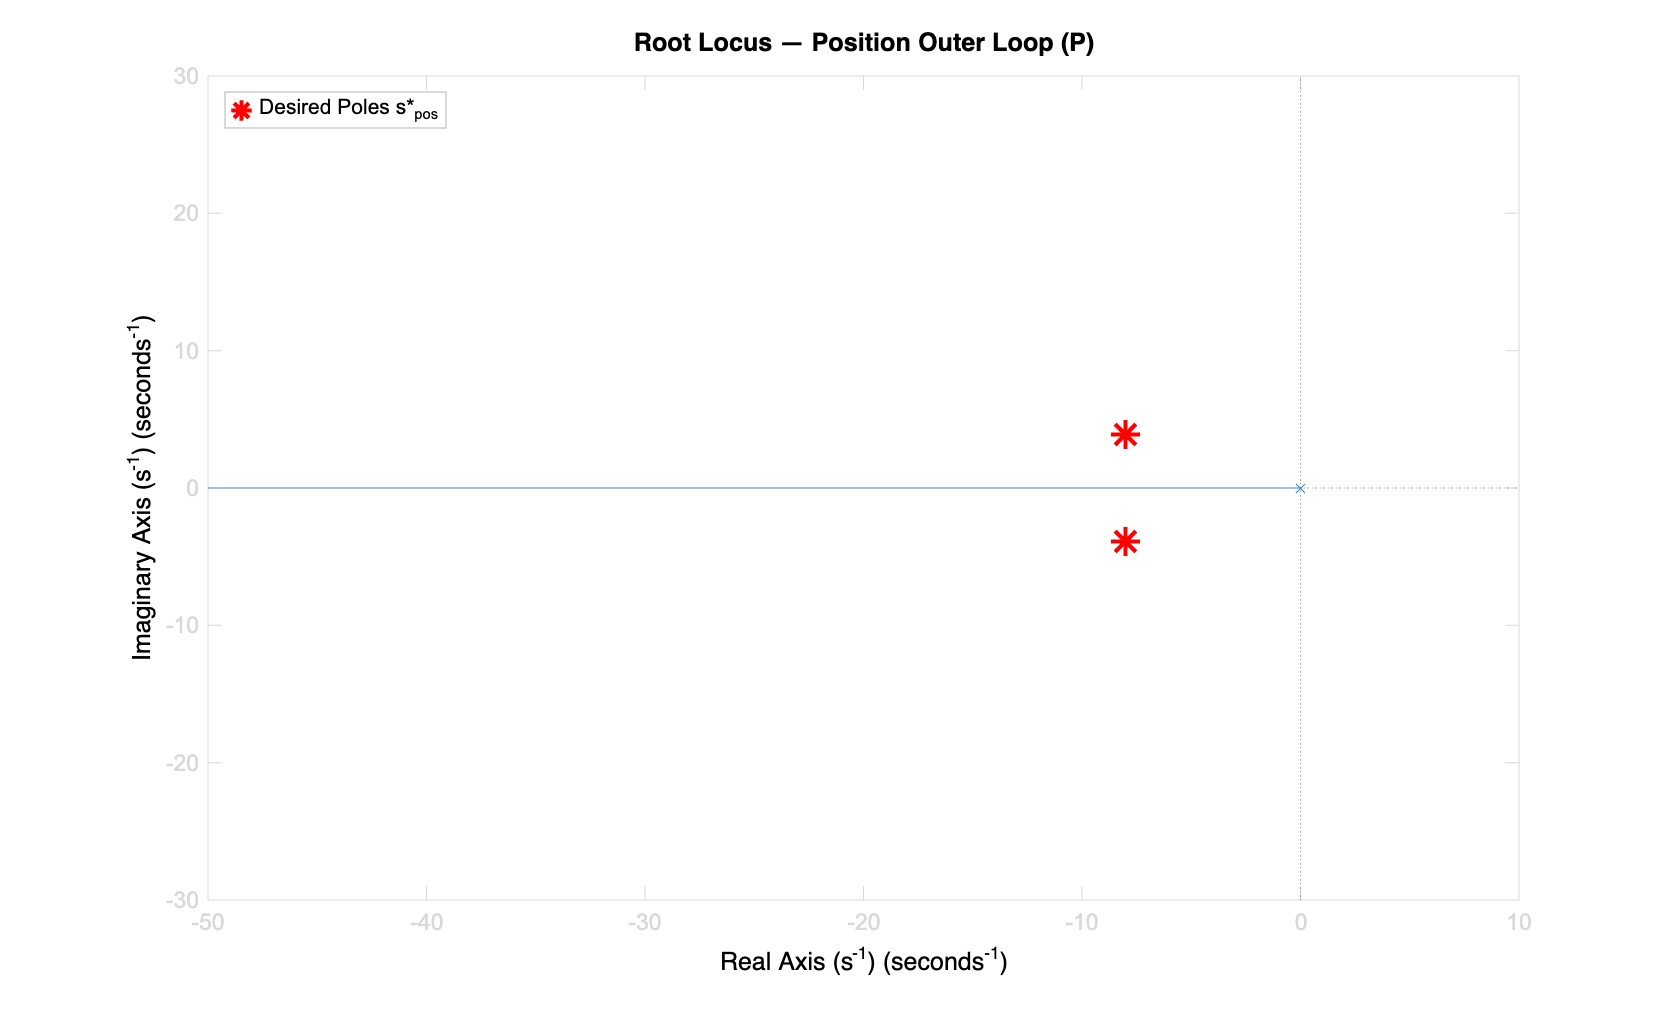
\includegraphics[width=1\textwidth]{fig_rlocus_position}
    \caption{Root Locus ของ Position Outer Loop (P + Integrator Plant)
             แสดง Desired Poles $s^*_{pos} = -8.000 \pm j3.875$
             (เครื่องหมาย $\times$ สีแดง) บนเส้น Damping Ratio
             $\zeta = 0.9$ (เส้นประสีน้ำเงิน)}
    \label{fig:rlocus_position}
\end{figure}

% -----------------------------------------------------------------------
\subsubsection{Anti-windup และ Feedforward}
% -----------------------------------------------------------------------

\paragraph{Anti-windup Back-calculation}

Velocity Loop มี $K_{i,vel}$ ขนาดใหญ่
ทำให้เมื่อเกิด Large Setpoint Change
Integrator State สะสมค่าสูงก่อนที่แรงดัน Output
จะถึง Saturation Limit $\pm 24$\,V (Integral Windup)
Anti-windup แบบ Back-calculation แก้ปัญหานี้
โดยป้อนกลับส่วนต่างระหว่าง Unsaturated
และ Saturated Output มาลด Integrator State
ตามที่อธิบายใน\cref{eq:anti_windup}

\begin{equation}
    K_{t,aw} = \frac{K_{i,vel}}{K_{p,vel}}
             = \frac{3512.963}{68.940}
             = 50.958\,\text{s}^{-1}
    \label{eq:Ktaw}
\end{equation}

\paragraph{Feedforward Gains}

Feedforward ช่วยลด Tracking Error ระหว่างการเคลื่อนที่
โดยไม่ต้องรอ Error สะสมก่อน
ระบบนี้มี Feedforward 3 ช่องทาง

\textbf{Velocity Feedforward ($K_{vff}$):}
ในสภาวะ Steady-State ที่ความเร็วคงที่
($\dot{\omega} = 0$, $\tau_d = 0$)
แทนค่าลงใน\cref{eq:mechanical_ode} และ\cref{eq:electrical_ode}
ได้แรงดันที่จำเป็น

\begin{equation}
    K_{vff} = \frac{R_a\,B}{\eta\,N\,K_t} + K_b\,N
            = \frac{1.4534 \times 0.19279}{0.836 \times 70 \times 0.04065}
              + 0.04165 \times 70
            = 0.117 + 2.916
            = 3.033\,\text{V/(rad/s)}
    \label{eq:kvff}
\end{equation}

\textbf{Acceleration Feedforward ($K_{aff}$):}
ในสภาวะที่มีความเร่ง $\dot{\omega} \neq 0$
แรงบิดส่วนที่ใช้เร่งมวล $J\dot{\omega}$
ต้องการแรงดันเพิ่มเติม

\begin{equation}
    K_{aff} = \frac{R_a\,J}{\eta\,N\,K_t}
            = \frac{1.4534 \times 0.72762}{0.836 \times 70 \times 0.04065}
            = \frac{1.0577}{2.376}
            = 0.445\,\text{V/(rad/s}^2\text{)}
    \label{eq:kaff}
\end{equation}

\textbf{Torque Disturbance Feedforward ($K_{tff}$):}
หาก Kalman Filter ประมาณค่า Disturbance Torque $\hat{\tau}_d$
ได้แล้ว สามารถชดเชยล่วงหน้าได้โดย

\begin{equation}
    \begin{aligned}
        K_{tff} &= \frac{R_a}{\eta \, N \, K_t} \\
                &= \frac{1.4534}{0.836 \times 70 \times 0.04065} \\
                &= \frac{1.4534}{2.376} \\
                &= 0.612 \, \mathrm{V/(N \cdot m)}
    \end{aligned}
    \label{eq:ktff}
\end{equation}

\noindent โดย $K_{tff}$ เปิดใช้งานเมื่อ Kalman Filter
Converge แล้วเท่านั้น ตามที่อธิบายใน\cref{subsec:kalman_filter}

\begin{table}[H]
  \centering
  \caption{สรุปค่า PID Gain และ Feedforward ของระบบควบคุม}
  \label{tab:pid_gains}
  \begin{tabular}{llccc}
    \toprule
    Loop & Gain & สัญลักษณ์ & ค่า & หน่วย \\
    \midrule
    \multirow{2}{*}{Velocity Inner (PI)}
      & Proportional & $K_{p,vel}$ & 68.940   & V/(rad/s) \\
      & Integral     & $K_{i,vel}$ & 3512.963 & V/rad \\
    \midrule
    Anti-windup
      & Back-calc    & $K_{t,aw}$  & 50.958   & s$^{-1}$ \\
    \midrule
    Position Outer (P)
      & Proportional & $K_{p,pos}$ & 8.889    & (rad/s)/rad \\
    \midrule
    \multirow{3}{*}{Feedforward}
      & Velocity FF      & $K_{vff}$ & 3.033 & V/(rad/s) \\
      & Acceleration FF  & $K_{aff}$ & 0.445 & V/(rad/s$^2$) \\
      & Disturbance FF   & $K_{tff}$ & 0.612 & V/(N$\cdot$m) \\
    \bottomrule
    \multicolumn{5}{l}{\small หมายเหตุ: $K_{vff}$, $K_{aff}$, $K_{tff}$
      ปิดระหว่าง Commissioning} \\
    \multicolumn{5}{l}{\small จนกว่า SysID uncertainty $< 10\%$
      และ Kalman Filter Converge} \\
  \end{tabular}
\end{table}

% -----------------------------------------------------------------------
\subsubsection{Hardware Commissioning และค่า Gain จริง}
\label{subsubsec:hw_commissioning}
% -----------------------------------------------------------------------

ค่า Gain ที่ได้จาก Pole Placement ใน\cref{eq:Kpv,eq:Kiv,eq:Kpp}
คำนวณภายใต้สมมติฐานว่าแบบจำลอง Plant มีความแม่นยำสมบูรณ์
และ Output ของ Controller คือแรงดัน $V_a$ ในหน่วย Volt
อย่างไรก็ตาม Firmware จริงบน STM32G474RE
ส่งคำสั่งในรูป PWM Count ($0$ ถึง $\pm$50)
ผ่านฟังก์ชัน \texttt{Motor\_SetPWM()} โดยมี Scale Factor

\begin{equation}
    \text{Scale} = \frac{V_{supply}}{PWM_{max}}
                 = \frac{24}{50}
                 = 0.48\,\text{V/PWM}
    \label{eq:pwm_scale}
\end{equation}

ดังนั้น Theoretical Gains ที่แปลงหน่วยเป็น PWM Unit แล้วคือ

\begin{equation}
    K_{p,vel}^{theory,hw}
        = \frac{K_{p,vel}^{theory}}{\text{Scale}}
        = \frac{68.940}{0.48}
        \approx 143.6\,\text{PWM/(rad/s)}
    \label{eq:Kpv_scaled}
\end{equation}

ซึ่งยังคงสูงกว่าค่าที่ใช้งานได้จริงอย่างมีนัยสำคัญ
เนื่องจากปัจจัยหลักสามประการ ได้แก่

\begin{itemize}
    \item \textbf{Model Uncertainty:}
          พารามิเตอร์ $J = 0.728\,\text{kg·m}^2$ และ $B = 0.193\,\text{N·m·s/rad}$
          ประมาณจาก Chirp Excitation ที่ความถี่ต่ำ (0.1--2\,Hz)
          ซึ่งอาจไม่สะท้อน Dynamic ของระบบที่ Bandwidth สูงกว่าได้อย่างแม่นยำ

    \item \textbf{Nonlinearity:}
          แบบจำลอง LTI ละทิ้ง Static Friction ของ Bearing และ Belt Drive
          ซึ่งมีผลต่อ Gain ที่เหมาะสมในสภาวะ Low-Velocity

    \item \textbf{PWM Saturation:}
          Gain สูงทำให้ Controller Output Saturate ที่ $\pm$50 PWM
          ในช่วง Transient เกือบตลอดเวลา
          ทำให้ระบบไม่ทำงานในย่าน Linear ตามที่ Pole Placement สมมติ
\end{itemize}

ด้วยเหตุนี้ Theoretical Gains จึงใช้เป็น \textbf{Order-of-Magnitude Reference}
และ \textbf{Starting Point} สำหรับ Hardware Commissioning เท่านั้น
ไม่ใช่ค่าที่นำไปใช้งานโดยตรง

\paragraph{ขั้นตอน Hardware Commissioning}

ดำเนินการ Tune Gains บน Hardware จริงตามลำดับดังนี้

\begin{enumerate}
    \item \textbf{Velocity Loop ก่อน:}
          ปิด Position Loop ชั่วคราว
          เพิ่ม $K_{p,vel}$ ทีละน้อยจนระบบเริ่ม Oscillate
          บันทึก $K_{p,crit}$ แล้วลดลงเหลือประมาณ $0.5 \times K_{p,crit}$
          จากนั้นเพิ่ม $K_{i,vel}$ ช้าๆ จนกำจัด Steady-State Error ได้

    \item \textbf{Position Loop ถัดไป:}
          เปิด Position Loop แล้วเพิ่ม $K_{p,pos}$ ทีละน้อย
          จนได้ Response ที่เร็วเพียงพอโดยไม่มี Overshoot
          จากนั้นปรับ $K_{d,pos}$ เพื่อ Damp การสั่น
          และ $K_{i,pos}$ เพื่อกำจัด Steady-State Error จาก Friction

    \item \textbf{ตรวจสอบ Requirements:}
          วัด Settling Time และ Overshoot จากการทดสอบ Step Response
          บน Hardware จริง เทียบกับ P5 ($t_s \leq 0.5$\,s)
          และ P6 (\%OS $\leq 1\%$)
\end{enumerate}

\subsection{ค่า Gain ที่ใช้งานจริง (Hardware-Tuned)}

\begin{table}[H]
  \centering
  \caption{เปรียบเทียบค่า PID Gain จาก Theoretical Design
           และ Hardware Commissioning}
  \label{tab:pid_gains_comparison}
  \begin{tabular}{llcccc}
    \toprule
    Loop & สัญลักษณ์ & Theoretical & Hardware & หน่วย (Theory) & หน่วย (HW) \\
    \midrule
    \multirow{2}{*}{Velocity (PI)}
      & $K_{p,vel}$ & 68.940   & [HW\_KPV] & V/(rad/s)      & PWM/(rad/s) \\
      & $K_{i,vel}$ & 3512.963 & [HW\_KIV] & V/rad          & PWM/rad     \\
    \midrule
    \multirow{3}{*}{Position (PID)}
      & $K_{p,pos}$ & 8.889  & [HW\_KPP] & (rad/s)/rad & (rad/s)/rad \\
      & $K_{i,pos}$ & --     & [HW\_KIP] & --          & (rad/s)/(rad·s) \\
      & $K_{d,pos}$ & --     & [HW\_KDP] & --          & (rad/s)·s/rad \\
    \midrule
    Anti-windup
      & $K_{t,aw}$  & 50.958 & [HW\_KAW] & s$^{-1}$ & s$^{-1}$ \\
    \midrule
    \multirow{3}{*}{Feedforward}
      & $K_{vff}$ & 3.033 & [HW\_KVFF] & V/(rad/s)     & PWM/(rad/s) \\
      & $K_{aff}$ & 0.445 & [HW\_KAFF] & V/(rad/s$^2$) & PWM/(rad/s$^2$) \\
      & $K_{tff}$ & 0.612 & [HW\_KTFF] & V/(N·m)       & PWM/(N·m) \\
    \bottomrule
    \multicolumn{6}{l}{\small [HW\_*] = ค่าที่ได้จาก Hardware Commissioning
      — อัปเดตหลัง Tuning เสร็จสิ้น} \\
  \end{tabular}
\end{table}

% -----------------------------------------------------------------------
% รูปที่: Step Response จาก Hardware Commissioning
% ชื่อไฟล์แนะนำ: fig_step_response_hw.png
% เนื้อหา: กราฟ Position (deg) vs Time (s) แสดง Step Response จริง
%          บน Hardware พร้อม annotation Settling Time และ Overshoot
%          เปรียบเทียบ Reference (เส้นประ) กับ Actual (เส้นทึบ)
% -----------------------------------------------------------------------
% \begin{figure}[H]
%     \centering
%     
\includegraphics[width=0.85\textwidth]{fig_step_response_hw}
%     \caption{Step Response ของระบบ Cascade PID บน Hardware จริง
%              แสดง Settling Time และ Overshoot
%              เทียบกับข้อกำหนด P5 ($t_s \leq 0.5$\,s)
%              และ P6 (\%OS $\leq 1\%$)}
%     \label{fig:step_response_hw}
% \end{figure}

\begin{table}[H]
  \centering
  \caption{ผลการทดสอบ Step Response บน Hardware
           เทียบกับ Requirements}
  \label{tab:hw_step_results}
  \begin{tabular}{lcccc}
    \toprule
    Metric & ผล Hardware & Requirement & หน่วย & สถานะ \\
    \midrule
    Settling Time  & [HW\_TS]  & $\leq 0.5$ & s   & [STATUS\_P5] \\
    Overshoot      & [HW\_OS]  & $\leq 1$   & \%  & [STATUS\_P6] \\
    Steady-State Error & [HW\_SSE] & --      & deg & -- \\
    \bottomrule
    \multicolumn{5}{l}{\small [HW\_*] = อัปเดตหลังเก็บข้อมูลจาก Hardware} \\
  \end{tabular}
\end{table}

% \subsubsection{ผลการ Simulation}

% \begin{table}[H]
%   \centering
%   \caption{ผลการ Simulation Cascade PID เปรียบเทียบกับ Requirements}
%   \label{tab:sim_results}
%   \begin{tabular}{lcccc}
%     \toprule
%     Metric & Unshaped & ZV-Shaped & Requirement & สถานะ \\
%     \midrule
%     Settling Time (Arm)  & 0.450\,s & 0.450\,s & $\leq 0.5$\,s & \textbf{PASS} \\
%     Overshoot            & 0.00\%   & 0.00\%   & $\leq 1\%$    & \textbf{PASS} \\
%     Steady-state Error   & $0.004°$ & $0.004°$ & --            & -- \\
%     Rod Peak Deflection  & $21.7°$  & $9.9°$   & $\leq 0.57°$ (at rest) & -- \\
%     Rod Settling Time    & 6.44\,s  & $\approx 0$\,s & -- & -- \\
%     \bottomrule
%   \end{tabular}
% \end{table}

% -----------------------------------------------------------------------
\subsubsection{การ Discretize สู่ Z-Domain (Tustin Transform)}
\label{subsubsec:discretization}
% -----------------------------------------------------------------------

การ Implement ตัวควบคุม Cascade PID บน STM32G474RE
จำเป็นต้องแปลง Continuous-time Controller
ให้เป็น Discrete-time ก่อน
โดยใช้วิธี Tustin (Bilinear Transform)

\begin{equation}
    s \;\longleftarrow\; \frac{2}{T}\cdot\frac{z-1}{z+1}
    \label{eq:tustin_sub}
\end{equation}

เหตุผลที่เลือก Tustin แทน Forward Euler ได้แก่
Tustin Map โพลทุกตัวในครึ่งซ้ายของระนาบ $s$
ให้อยู่ภายใน Unit Circle ของระนาบ $z$ อย่างสมบูรณ์
ในขณะที่ Forward Euler อาจทำให้ Discrete System
ไม่เสถียรแม้ Continuous System จะเสถียร
โดยเฉพาะเมื่อ $K_i/f_s$ มีขนาดใหญ่
ตามที่อธิบายใน\cref{subsec:cascade_pid}

% -----------------------------------------------------------------------
\paragraph{Velocity Inner Loop — PI (Tustin)}
% -----------------------------------------------------------------------

Continuous-time PI Controller ของ Velocity Loop คือ

\begin{equation}
    C_v(s) = K_{p,vel} + \frac{K_{i,vel}}{s}
    \label{eq:Cv_ct}
\end{equation}

แทน\cref{eq:tustin_sub} ลงใน\cref{eq:Cv_ct}
ที่ Sample Time $T_v = 1$\,ms ได้

\begin{equation}
    C_v(z) = K_{p,vel}
           + K_{i,vel}\cdot\frac{T_v}{2}\cdot\frac{z+1}{z-1}
    \label{eq:Cv_z}
\end{equation}

จัดรูปให้ได้ Difference Equation
โดยกำหนด $u_v[k]$ เป็น PWM Output
และ $e_v[k] = \omega_{sp}[k] - \omega_{act}[k]$
เป็น Velocity Error

\begin{equation}
    u_v[k] = u_v[k-1]
           + \underbrace{\left(K_{p,vel} + \frac{K_{i,vel}\,T_v}{2}\right)}_{c_1}
             e_v[k]
           + \underbrace{\left(-K_{p,vel} + \frac{K_{i,vel}\,T_v}{2}\right)}_{c_2}
             e_v[k-1]
    \label{eq:vel_diff_eq}
\end{equation}

\noindent โดยที่

\begin{align}
    c_1 &= K_{p,vel} + \frac{K_{i,vel}\,T_v}{2}
         = 68.940 + \frac{3512.963 \times 0.001}{2}
         = 68.940 + 1.756
         = 70.696
    \label{eq:c1_vel} \\[4pt]
    c_2 &= -K_{p,vel} + \frac{K_{i,vel}\,T_v}{2}
         = -68.940 + 1.756
         = -67.184
    \label{eq:c2_vel}
\end{align}

Difference Equation นี้ implement ได้โดยตรงใน Firmware
โดยเก็บเพียง $u_v[k-1]$ และ $e_v[k-1]$
เป็น Static Variable ซึ่งมี Memory Footprint
เพียง 2 ตัวแปร Float (8 bytes) ต่อ Loop

% -----------------------------------------------------------------------
\paragraph{Position Outer Loop — PID (Tustin, Derivative on Measurement)}
% -----------------------------------------------------------------------

Continuous-time PID Controller ของ Position Loop คือ

\begin{equation}
    C_p(s) = K_{p,pos} + \frac{K_{i,pos}}{s} + K_{d,pos}\,s
    \label{eq:Cp_ct}
\end{equation}

แทน Tustin Transform ที่ $T_p = 10$\,ms
และใช้ Derivative on Measurement
(แทน Derivative on Error เพื่อป้องกัน Derivative Kick
เมื่อ Setpoint เปลี่ยนแบบ Step)

\begin{equation}
    \text{D-term} = -K_{d,pos}\,\frac{d\theta_{act}}{dt}
    \label{eq:d_on_meas}
\end{equation}

Difference Equation ของ Position PID คือ

\begin{align}
    u_p[k] &= K_{p,pos}\,e_p[k] \notag \\
            &+ \frac{K_{i,pos}\,T_p}{2}
               \bigl(e_p[k] + e_p[k-1]\bigr)
               + I_p[k-1] \notag \\
            &- K_{d,pos}\,\frac{\theta_{act}[k] - \theta_{act}[k-1]}{T_p}
    \label{eq:pos_diff_eq}
\end{align}

\noindent โดยที่ $I_p[k]$ คือ Integral State ที่ Update ตาม

\begin{equation}
    I_p[k] = I_p[k-1]
           + \frac{K_{i,pos}\,T_p}{2}
             \bigl(e_p[k] + e_p[k-1]\bigr)
    \label{eq:pos_integral_update}
\end{equation}

และ $u_p[k]$ คือ Velocity Setpoint
ที่ส่งเข้า Velocity Inner Loop
ซึ่ง Clamp ไว้ที่ $\pm v_{max} = \pm 7.304$\,rad/s

% -----------------------------------------------------------------------
\paragraph{Anti-windup ใน Discrete-time}
% -----------------------------------------------------------------------

ทั้งสอง Loop ใช้ Conditional Integration
เพื่อป้องกัน Integral Windup โดย

\begin{itemize}
    \item \textbf{Velocity Loop:}
          หยุด Integrate เมื่อ Feedforward Output
          ใกล้ Saturation Limit
          ($|u_{ff}| \geq PWM_{max} - 1$)
          เนื่องจากสภาวะดังกล่าว PID Output
          จะถูก Clamp อยู่ดีและ Integral State
          ที่สะสมต่อไปจะไม่มีผลต่อ Output จริง

    \item \textbf{Position Loop:}
          หยุด Integrate เมื่อ Position Error
          อยู่ภายใน Deadband
          ($|e_p| < \delta_{dead}$)
          ป้องกัน Windup ขณะจอดนิ่ง
\end{itemize}

% -----------------------------------------------------------------------
\begin{table}[H]
  \centering
  \caption{สรุปค่าสัมประสิทธิ์ Discrete-time Controller
           (Theoretical Gains, หน่วย V)}
  \label{tab:discrete_coeffs}
  \begin{tabular}{llccc}
    \toprule
    Loop & พารามิเตอร์ & สัญลักษณ์ & ค่า & หน่วย \\
    \midrule
    \multirow{4}{*}{Velocity PI}
      & Sample Time       & $T_v$  & 0.001   & s \\
      & Forward Coeff     & $c_1$  & 70.696  & V/(rad/s) \\
      & Backward Coeff    & $c_2$  & $-67.184$ & V/(rad/s) \\
      & Integral Clamp    & $I_{max,v}$ & \texttt{PID\_SPEED\_IMAX} & V \\
    \midrule
    \multirow{4}{*}{Position PID}
      & Sample Time       & $T_p$  & 0.010  & s \\
      & Proportional      & $K_{p,pos}$ & 8.889 & (rad/s)/rad \\
      & Integral Step     & $K_{i,pos}T_p/2$ & [HW\_KIP\_STEP] & (rad/s)/rad \\
      & Derivative        & $K_{d,pos}/T_p$ & [HW\_KDP\_RATE] & (rad/s)·s/rad \\
    \bottomrule
    \multicolumn{5}{l}{\small หมายเหตุ: ค่า [HW\_*] อัปเดตหลัง Hardware Commissioning} \\
  \end{tabular}
\end{table}

\begin{figure}[H]
    \centering
    
\includegraphics[width=0.90\textwidth]{fig_zpole_cascade}
    \caption{Pole-Zero Map ใน Z-Domain ของ Velocity PI (ซ้าย)
             และ Position PID (ขวา) หลัง Tustin Discretization
             Poles และ Zeros ทั้งหมดอยู่ภายใน Unit Circle
             ยืนยันความเสถียรของ Discrete-time Controller}
    \label{fig:zpole_cascade}
\end{figure}

\begin{figure}[H]
    \centering
    
\includegraphics[width=0.90\textwidth]{fig_bode_discretization}
    \caption{Bode Plot เปรียบเทียบ Continuous-time (สีเทา),
             Tustin (สีน้ำเงิน) และ Forward Euler (สีแดง)
             แสดงว่า Tustin ให้ Frequency Response
             ใกล้เคียง Continuous ในย่าน Passband
             ในขณะที่ Forward Euler มี Phase Error
             สูงกว่าเมื่อความถี่เข้าใกล้ $f_{Nyquist}$}
    \label{fig:bode_discretization}
\end{figure}

% -----------------------------------------------------------------------
\subsubsection{การวิเคราะห์เสถียรภาพในโดเมนความถี่}
\label{subsubsec:frequency_analysis}
% -----------------------------------------------------------------------

การวิเคราะห์เสถียรภาพของ Cascade PID ดำเนินการใน
Frequency Domain โดยใช้ Open-loop Bode Plot
เพื่อหา Gain Margin (GM) และ Phase Margin (PM)
ซึ่งเป็น Stability Margin มาตรฐานสำหรับ
Linear Feedback System
เกณฑ์ขั้นต่ำที่ยอมรับได้ทั่วไปคือ
GM $> 6$\,dB และ PM $> 30°$

\begin{figure}[H]
    \centering
    
\includegraphics[width=0.85\textwidth]{fig_bode_openloop_vel}
    \caption{Open-Loop Bode Plot ของ Velocity Inner Loop
             แสดง Phase Margin ที่ Gain Crossover Frequency
             ยืนยันความเสถียรของ Velocity Loop}
    \label{fig:bode_openloop_vel}
\end{figure}

\begin{figure}[H]
    \centering
    
\includegraphics[width=0.85\textwidth]{fig_bode_openloop_pos}
    \caption{Open-Loop Bode Plot ของ Position Outer Loop (Cascade)
             แสดง Gain Margin และ Phase Margin
             ของระบบ Cascade รวมทั้งสอง Loop}
    \label{fig:bode_openloop_pos}
\end{figure}

\begin{table}[H]
  \centering
  \caption{สรุป Stability Margin ของ Cascade PID}
  \label{tab:stability_margin}
  \begin{tabular}{lcccc}
    \toprule
    Loop & GM (dB) & PM (deg) & $f_{cp}$ (Hz) & สถานะ \\
    \midrule
    Velocity Inner & $\infty$ & 74.64 & 25.58 & \textbf{ผ่าน} \\
    Position Outer & $\infty$ & 98.07 &  1.46 & \textbf{ผ่าน} \\
    \bottomrule
    \multicolumn{5}{l}{\small เกณฑ์: GM $> 6$\,dB และ PM $> 30°$} \\
  \end{tabular}
\end{table}

\begin{figure}[H]
    \centering
    
\includegraphics[width=0.90\textwidth]{fig_bode_sensitivity}
    \caption{Closed-loop Frequency Response แสดง
             Complementary Sensitivity $T(s)$ (บน)
             และ Sensitivity $S(s)$ (ล่าง)
             ของ Velocity Loop (ซ้าย) และ Position Loop (ขวา)
             เส้นประแสดงจุด $-3$\,dB Bandwidth ของแต่ละ Loop}
    \label{fig:bode_sensitivity}
\end{figure}

Gain Margin มีค่าเป็น $\infty$ ในทั้งสอง Loop
เนื่องจาก Phase ของ Open-loop Transfer Function
ไม่เคยลดลงถึง $-180°$ ในย่านความถี่ใด
ซึ่งเป็นลักษณะปกติของระบบ PI และ PID
ที่มี Integrator เพียงหนึ่งตัวใน Loop
ดังนั้น Phase Margin จึงเป็น Stability Indicator
หลักของระบบนี้

Phase Margin ของ Velocity Loop ($74.6°$)
และ Position Loop ($98.1°$) สูงกว่าเกณฑ์ขั้นต่ำ
$30°$ อย่างมีนัยสำคัญ
แสดงว่าระบบมี Stability Margin เพียงพอ
และสามารถรองรับ Plant Model Uncertainty
ได้ในระดับสูง

Gain Crossover Frequency ของ Velocity Loop
ที่ $f_{cp} = 25.58$\,Hz ยืนยัน Bandwidth
Separation จาก Position Loop ($f_{cp} = 1.46$\,Hz)
ที่อัตราส่วน $25.58/1.46 \approx 17.5$ เท่า
ซึ่งเกินกว่าเกณฑ์ 10 เท่าที่ออกแบบไว้
ตาม\cref{eq:bw_sep}

% ============================================================================
\subsection{การออกแบบ ZVD Input Shaper}
\label{subsec:zv_design}
% ============================================================================

% -----------------------------------------------------------------------
\subsubsection{แบบจำลอง Connection Rod และเหตุผลที่ต้องใช้ Input Shaping}
\label{subsubsec:rod_model}
% -----------------------------------------------------------------------

Connection Rod มีมวล $m_{rod} = 164.08$\,g และความยาว $L_{rod} = 100$\,mm
จำลองเป็น Simple Pendulum ที่ถูกกระตุ้นด้วย Angular Acceleration
ของแขนกล $\alpha_{arm}$ ตามที่อธิบายใน\cref{subsec:rod_dynamics}
สมการการเคลื่อนที่ในรูปแบบ Standard 2nd-order ได้จาก\cref{eq:rod_eom}

\begin{equation}
    \ddot{\phi} + 2\zeta_{rod}\,\omega_{n,rod}\,\dot{\phi}
    + \omega_{n,rod}^2\,\phi
    = \underbrace{-\frac{3\,r_{arm}}{2\,L_{rod}}}_{\Gamma}\,\alpha_{arm}
    \label{eq:rod_eom_ch3}
\end{equation}

\noindent โดยที่ $\Gamma = -3 \times 0.5 / (2 \times 0.1) = -7.5$
คือ Forcing Gain และความถี่ธรรมชาติคำนวณได้จาก\cref{eq:rod_natural_freq}

\begin{equation}
    \omega_{n,rod} = \sqrt{\frac{3g}{2L_{rod}}}
                   = \sqrt{\frac{3 \times 9.81}{2 \times 0.1}}
                   = 12.131\,\text{rad/s}
                   \quad (f_n = 1.931\,\text{Hz})
    \label{eq:rod_wn_ch3}
\end{equation}

ค่า Damping Ratio $\zeta_{rod} = 0.041$ ใช้เป็น Conservative Assumption
สำหรับ Lightly Damped Mechanical System
ซึ่งให้ Settling Time ต่อ Move ที่

\begin{equation}
    t_{settle,rod} \approx \frac{4}{\zeta_{rod}\,\omega_{n,rod}}
                         = \frac{4}{0.041 \times 12.131}
                         = 8.04\,\text{s/move}
    \label{eq:rod_settle}
\end{equation}

หากระบบมี 9 Moves ต่อ Cycle และต้องรอให้ Rod หยุดแกว่งก่อนทุก Move
Cycle Time รวมจะเกิน $9 \times 8.04 = 72.4$\,s
ซึ่งเกินข้อกำหนด P1 ($\leq 35$\,s) อย่างมาก
การใช้ Input Shaper จึงเป็นข้อกำหนดที่ขาดไม่ได้

% -----------------------------------------------------------------------
\subsubsection{การออกแบบ ZVD Input Shaper (3-Impulse)}
\label{subsubsec:zvd_design}
% -----------------------------------------------------------------------

ระบบเลือกใช้ ZVD (Zero-Vibration-Derivative) Shaper แบบ 3-Impulse
แทน ZV แบบ 2-Impulse เนื่องจาก ZVD มีเงื่อนไขเพิ่มเติม
ว่า Derivative ของ Residual Vibration เทียบกับ $\omega_n$
ต้องเป็นศูนย์ด้วย ทำให้ทนทานต่อความไม่แน่นอนของ $\omega_n$
ได้สูงกว่า ดังที่จะเห็นใน\cref{fig:zvd_sensitivity}

\paragraph{การคำนวณพารามิเตอร์ ZVD}

กำหนดค่า Decay Factor

\begin{equation}
    K = e^{-\zeta_{rod}\pi/\sqrt{1-\zeta_{rod}^2}}
      = e^{-0.041\pi/\sqrt{1-0.041^2}}
      = e^{-0.1288}
      = 0.8790
    \label{eq:zvd_K}
\end{equation}

แอมพลิจูดของ Impulse ทั้งสามคำนวณจาก\cref{eq:zv_amplitudes}

\begin{align}
    A_1 &= \frac{1}{(1+K)^2}
         = \frac{1}{(1.8790)^2}
         = 0.2832
    \label{eq:zvd_A1} \\[4pt]
    A_2 &= \frac{2K}{(1+K)^2}
         = \frac{2 \times 0.8790}{(1.8790)^2}
         = 0.4979
    \label{eq:zvd_A2} \\[4pt]
    A_3 &= \frac{K^2}{(1+K)^2}
         = \frac{(0.8790)^2}{(1.8790)^2}
         = 0.2189
    \label{eq:zvd_A3}
\end{align}

ตรวจสอบ: $A_1 + A_2 + A_3 = 0.2832 + 0.4979 + 0.2189 = 1.0000$ \checkmark

Impulse Delay คำนวณจาก Half-Period ของ Damped Oscillation

\begin{equation}
    T_d = \frac{\pi}{\omega_{n,rod}\sqrt{1-\zeta_{rod}^2}}
        = \frac{\pi}{12.131 \times \sqrt{1-0.041^2}}
        = \frac{\pi}{12.121}
        = 0.2592\,\text{s}
    \label{eq:zvd_Td}
\end{equation}

\begin{equation}
    t_2 = T_d = 0.2592\,\text{s}
    \quad (26\;\text{steps @ 100\,Hz}),
    \qquad
    t_3 = 2T_d = 0.5184\,\text{s}
    \quad (52\;\text{steps @ 100\,Hz})
    \label{eq:zvd_delays}
\end{equation}

% -----------------------------------------------------------------------
% รูปที่: ZVD Impulse Sequence
% ชื่อไฟล์: fig_zvd_impulse_sequence.png
% -----------------------------------------------------------------------
\begin{figure}[H]
    \centering
    
\includegraphics[width=0.75\textwidth]{fig_zvd_impulse_sequence}
    \caption{ZVD 3-Impulse Sequence แสดงแอมพลิจูด $A_1$, $A_2$, $A_3$
             และเวลาหน่วง $t_2 = 0.259$\,s ($26$ steps)
             และ $t_3 = 0.518$\,s ($52$ steps) ที่ Outer Loop 100\,Hz}
    \label{fig:zvd_impulse_sequence}
\end{figure}

\begin{table}[H]
  \centering
  \caption{พารามิเตอร์ ZVD Input Shaper ที่ใช้ใน Firmware}
  \label{tab:zvd_params}
  \begin{tabular}{llll}
    \toprule
    พารามิเตอร์ & สัญลักษณ์ & ค่า & หมายเหตุ \\
    \midrule
    Natural Frequency & $\omega_{n,rod}$ & 12.131\,rad/s & คำนวณจาก\cref{eq:rod_wn_ch3} \\
    Damping Ratio     & $\zeta_{rod}$    & 0.041         & Conservative Assumption \\
    Decay Factor      & $K$              & 0.8790        & \cref{eq:zvd_K} \\
    Impulse 1         & $A_1$            & 0.2832        & \cref{eq:zvd_A1} \\
    Impulse 2         & $A_2$            & 0.4979        & \cref{eq:zvd_A2} \\
    Impulse 3         & $A_3$            & 0.2189        & \cref{eq:zvd_A3} \\
    Delay 2           & $t_2$            & 0.2592\,s (26 steps) & \cref{eq:zvd_delays} \\
    Delay 3           & $t_3$            & 0.5184\,s (52 steps) & \cref{eq:zvd_delays} \\
    \bottomrule
  \end{tabular}
\end{table}

% -----------------------------------------------------------------------
\subsubsection{การวิเคราะห์ความทนทานต่อความไม่แน่นอนของความถี่}
\label{subsubsec:zvd_sensitivity}
% -----------------------------------------------------------------------

ในการใช้งานจริง ค่า $\omega_{n,rod}$ อาจเปลี่ยนแปลงได้
เนื่องจากน้ำหนักของ Connection Rod ที่แตกต่างกัน
หรือความยาวของ Rod ที่ไม่แน่นอน
\cref{fig:zvd_sensitivity} แสดง Residual Vibration
เมื่อ $\omega_{actual}$ ต่างจาก $\omega_{design}$
สำหรับ ZV (2-Impulse) และ ZVD (3-Impulse)

% -----------------------------------------------------------------------
% รูปที่: ZVD Sensitivity Analysis
% ชื่อไฟล์: fig_zvd_sensitivity.png
% -----------------------------------------------------------------------
\begin{figure}[H]
    \centering
    
\includegraphics[width=0.82\textwidth]{fig_zvd_sensitivity}
    \caption{Sensitivity Analysis เปรียบเทียบ ZV (สีแดง)
             และ ZVD (สีน้ำเงิน) แสดง Residual Vibration
             เมื่อ $\omega_{actual}/\omega_{design}$ เบี่ยงจาก 1.0
             ZVD รักษา Residual Vibration ต่ำกว่า 5\%
             ในย่านกว้างกว่า ZV อย่างมีนัยสำคัญ}
    \label{fig:zvd_sensitivity}
\end{figure}

จากกราฟ ZVD รักษา Residual Vibration ต่ำกว่า 5\%
ในย่าน $\omega_{actual}/\omega_{design} \in [0.88, 1.12]$
ในขณะที่ ZV รักษาได้เพียง $[0.94, 1.06]$
แสดงว่า ZVD ทนทานต่อความไม่แน่นอนของ $\omega_n$
ได้กว้างกว่าประมาณ 2 เท่า

% -----------------------------------------------------------------------
\subsubsection{ผลการ Simulation: Unshaped กับ ZVD-Shaped}
\label{subsubsec:zvd_results}
% -----------------------------------------------------------------------

\cref{fig:zvd_rod_response} แสดงผลการ Simulation
ของการแกว่ง Rod ในสภาวะ Worst-case
(Move 360° ด้วย S-curve ที่ $v_{max} = 7.304$\,rad/s,
$a_{max} = 27.49$\,rad/s$^2$, $j_{max} = 1400$\,rad/s$^3$)

% -----------------------------------------------------------------------
% รูปที่: Rod Swing Response
% ชื่อไฟล์: fig_zvd_rod_response.png
% -----------------------------------------------------------------------
\begin{figure}[H]
    \centering
    
\includegraphics[width=0.90\textwidth]{fig_zvd_rod_response}
    \caption{(ก) S-curve Acceleration Profile ของแขนกล
             Unshaped (สีเทา) และ ZVD-Shaped (สีน้ำเงิน)
             (ข) การแกว่งของ Connection Rod $\phi_{rod}$
             แสดง Settling Time ของ Unshaped
             และการยกเลิกการแกว่งของ ZVD-Shaped
             สำหรับ Worst-case Move 360°}
    \label{fig:zvd_rod_response}
\end{figure}

\begin{table}[H]
  \centering
  \caption{สรุปผลการ Simulation เปรียบเทียบ Unshaped กับ ZVD-Shaped
           (Worst-case Move 360°)}
  \label{tab:zv_comparison}
  \begin{tabular}{lccc}
    \toprule
    Metric & Unshaped & ZVD-Shaped & ผลต่าง \\
    \midrule
    Rod Peak Deflection  & $179.95°$ & $53.52°$   & $-70.3\%$ \\
    Rod Settling Time    & $0.21$\,s & $0.44$\,s  & -- \\
    Move Time            & $1.146$\,s & $1.146 + t_3 = 1.664$\,s & $+0.518$\,s \\
    \bottomrule
  \end{tabular}
\end{table}

\textbf{หมายเหตุเกี่ยวกับแบบจำลอง:}
การ Simulation ใช้ Nonlinear Pendulum Model
($\sin\phi$ แทน $\phi$) พร้อม Wrap-around
ที่ $\pm 180°$ เพื่อสะท้อนข้อจำกัดทางกายภาพจริง
อย่างไรก็ตามค่า Peak Deflection ของ Unshaped
ที่ $\approx 180°$ บ่งชี้ว่าใน Worst-case
(Move 360° ด้วย $a_{max} = 27.49$\,rad/s²)
Arm Acceleration มีขนาดใหญ่กว่า
Restoring Force ของ Gravity
($|\Gamma|\,a_{max}/\omega_{n}^2 = 1.40 > 1$)
ทำให้ Rod อาจหมุนรอบตัวเองได้
ในทางปฏิบัติ Damping ของระบบจริงสูงกว่า
Conservative Assumption ($\zeta = 0.041$) ที่ใช้ใน Simulation
และ Gripper จับ Rod ในลักษณะที่จำกัดการแกว่งบางส่วน
ดังนั้นผลการ Simulation จึงเป็น
\textbf{Conservative Worst-case Estimate}
และผลเปรียบเทียบเชิงสัดส่วนระหว่าง
Unshaped และ ZVD-Shaped ยังคงสื่อความหมายได้
กล่าวคือ ZVD ลด Peak Deflection ได้ $70.3\%$
โดยแลกกับ Delay เพิ่มเพียง $t_3 = 0.518$\,s ต่อ Move

ผลการ Simulation ยืนยันว่า ZVD Input Shaper
สามารถยกเลิกการแกว่งของ Rod ได้อย่างมีประสิทธิภาพ
โดยแลกกับ Delay เพิ่มเพียง $t_3 = 0.518$\,s ต่อ Move
ซึ่งน้อยกว่า Settling Time ของ Unshaped
($\approx 8$\,s) อย่างมีนัยสำคัญ
ทำให้ Cycle Time รวมอยู่ในเกณฑ์ P1 ($\leq 35$\,s)

% ============================================================================
\subsection{การออกแบบ S-Curve Motion Profile}
\label{subsec:scurve_design}
% ============================================================================

S-Curve Trajectory หรือ Jerk-Limited Trajectory
เป็นโปรไฟล์การเคลื่อนที่ที่จำกัดอัตราการเปลี่ยนแปลงของความเร่ง
(Jerk, $j = d^3\theta/dt^3$) ให้ไม่เกินค่าสูงสุด $j_{max}$
ซึ่งช่วยลดแรงกระชากทางกล (Mechanical Shock)
และจำกัดการกระตุ้นความถี่ธรรมชาติของระบบ
เมื่อเทียบกับ Trapezoidal Profile ที่มีค่า Jerk เป็นอนันต์
ณ จุดที่เปลี่ยนความเร่ง
ตามที่อธิบายใน\cref{subsec:scurve}

% -----------------------------------------------------------------------
\subsubsection{พารามิเตอร์ S-Curve จาก Hardware Identification}
\label{subsubsec:scurve_params}
% -----------------------------------------------------------------------

ขีดจำกัด Motion Profile วัดและระบุจาก Hardware จริง
แล้ว Hard-code ไว้ใน \texttt{params.h} ของ Firmware

\begin{equation}
    v_{max} = 7.304\,\text{rad/s}, \quad
    a_{max} = 27.49\,\text{rad/s}^2, \quad
    j_{max} = 1400\,\text{rad/s}^3
    \label{eq:scurve_limits}
\end{equation}

\subsubsection{การคำนวณ Phase Times}

S-Curve แบบสมมาตร (Symmetric Profile) แบ่งออกเป็น 7 เฟส
โดยมีเวลาในแต่ละ Phase คำนวณได้จาก\cref{eq:scurve_tj,eq:scurve_ta,eq:scurve_tv}

\begin{align}
    T_j &= \frac{a_{max}}{j_{max}}
         = \frac{27.49}{1400}
         = 0.0196\,\text{s}
    \label{eq:scurve_tj_num} \\[4pt]
    T_a &= \frac{v_{max}}{a_{max}} - T_j
         = \frac{7.304}{27.49} - 0.0196
         = 0.2461\,\text{s}
    \label{eq:scurve_ta_num} \\[4pt]
    T_v &= \frac{\Delta\theta - d_{acc,decel}}{v_{max}}
    \label{eq:scurve_tv_num}
\end{align}

\noindent โดยที่ $d_{acc,decel}$ คือระยะทางรวมในช่วง
Acceleration และ Deceleration
ค่า $T_v$ ขึ้นอยู่กับระยะทางเป้าหมาย $\Delta\theta$
ของแต่ละ Move

\begin{table}[H]
  \centering
  \caption{พารามิเตอร์ S-Curve Motion Profile จาก Hardware Identification}
  \label{tab:scurve_params}
  \begin{tabular}{llcc}
    \toprule
    พารามิเตอร์ & สัญลักษณ์ & ค่า & หน่วย \\
    \midrule
    Maximum Velocity    & $v_{max}$ & 7.304  & rad/s \\
    Maximum Acceleration & $a_{max}$ & 27.49  & rad/s$^2$ \\
    Maximum Jerk        & $j_{max}$ & 1400   & rad/s$^3$ \\
    Jerk Phase Time     & $T_j$     & 0.0196 & s \\
    Accel Phase Time    & $T_a$     & 0.2461 & s \\
    \bottomrule
    \multicolumn{4}{l}{\small $T_v$ ขึ้นกับระยะทางของแต่ละ Move}
  \end{tabular}
\end{table}

% =======================================================================
% แทรกรูป S-Curve Profile ของ 1 Move (Worst-case 360 deg) ตรงนี้
% =======================================================================
\begin{figure}[H]
    \centering
    
\includegraphics[width=\textwidth]{fig_scurve_profile}
    \caption{ลักษณะจำเพาะของ S-Curve Motion Profile สำหรับ 1 การเคลื่อนที่ (Worst-case 360°) 
             แสดงความสัมพันธ์ของ (ก)~Position (ข)~Velocity (ค)~Acceleration และ (ง)~Jerk 
             โดยแบ่งการทำงานออกเป็น 7 เฟส (P1-P7) ซึ่งแสดงให้เห็นถึงความต่อเนื่องของความเร่ง
             และการจำกัดอัตราการกระชาก (Jerk-limited) อย่างชัดเจน}
    \label{fig:scurve_single_profile}
\end{figure}
% =======================================================================

จาก\cref{fig:scurve_single_profile} พฤติกรรมการเคลื่อนที่แบบ S-Curve สำหรับ 1 คำสั่งการเคลื่อนที่ (Point-to-Point Move) สามารถแบ่งออกเป็น 7 เฟส (P1 ถึง P7) ตามการควบคุมอัตราการกระชาก (Jerk) ดังนี้:

\begin{itemize}
    \item \textbf{P1 (Jerk Up):} ระบบเริ่มจ่ายค่า Jerk สูงสุด ($+j_{max}$) ทำให้ความเร่งเพิ่มขึ้นแบบเชิงเส้นจากศูนย์จนถึงขีดจำกัด $+a_{max}$ ภายในเวลา $T_j$
    \item \textbf{P2 (Constant Acceleration):} ระบบรักษาความเร่งคงที่ระดับ $+a_{max}$ (Jerk เป็นศูนย์) ทำให้ความเร็วเพิ่มขึ้นแบบเชิงเส้นเป็นความชันคงที่
    \item \textbf{P3 (Jerk Down):} ระบบจ่าย Jerk ติดลบ ($-j_{max}$) เพื่อลดความเร่งลงกลับสู่ศูนย์อย่างนุ่มนวล ในเฟสนี้ความเร็วจะค่อยๆ ลู่เข้าสู่ขีดจำกัดสูงสุด $v_{max}$
    \item \textbf{P4 (Constant Velocity):} ช่วงวิ่งด้วยความเร็วคงที่ ($v_{max}$) ความเร่งและ Jerk มีค่าเป็นศูนย์ ระยะเวลาในเฟสนี้ ($T_v$) จะแปรผันตามระยะทางเป้าหมาย $\Delta\theta$ หากระยะทางสั้นเกินไป เฟสนี้อาจไม่มีอยู่จริง (กลายเป็น Triangular Profile)
    \item \textbf{P5 ถึง P7 (Deceleration Phase):} เป็นกระบวนการที่สะท้อนกลับ (Mirror) กับ P1 ถึง P3 โดยระบบจะสร้างความหน่วง (Negative Acceleration) สูงสุดที่ $-a_{max}$ เพื่อลดความเร็วลงจนหยุดนิ่งที่ตำแหน่งเป้าหมายอย่างแม่นยำ
\end{itemize}

\textbf{ข้อได้เปรียบเชิงวิศวกรรม (Engineering Advantages):} 
ความราบเรียบของความเร่งในช่วง P1, P3, P5 และ P7 คือหัวใจสำคัญของ S-Curve Profile การที่ความเร่งมีความต่อเนื่องทางคณิตศาสตร์ (Continuous Acceleration) จะช่วยหลีกเลี่ยงการเกิด Impulse Force ภายในกลไก ซึ่งส่งผลดีอย่างยิ่งยวดต่อระบบ Pick-and-Place ที่มี Connection Rod แบบยืดหยุ่นห้อยอยู่ เนื่องจากมันช่วยลดการกระตุ้นความถี่ธรรมชาติสูงๆ (High-frequency Excitation) ทำให้ขนาดของ Residual Vibration เริ่มต้นต่ำกว่าการใช้ Trapezoidal Profile อย่างมีนัยสำคัญ

% -----------------------------------------------------------------------
\subsubsection{การวิเคราะห์ Cycle Time}
\label{subsubsec:cycle_time}
% -----------------------------------------------------------------------

ทดสอบ Cycle Time ด้วย 2 Scenarios เพื่อครอบคลุม
ทั้งกรณี Worst-case และกรณีทั่วไป
โดยแต่ละ Cycle ประกอบด้วย 4 Pick-Place Pairs (9 Moves)
และ Gripper Time 2\,s ต่อ Station รวม 8 Stations

\begin{equation}
    t_{cycle} = \sum_{i=1}^{9} t_{move,i}
               + 8 \times t_{grip}
               = \sum_{i=1}^{9} t_{move,i} + 16\,\text{s}
    \label{eq:cycle_time}
\end{equation}

\paragraph{Scenario 1: Worst-case ($0° \leftrightarrow 360°$)}

แต่ละ Move ใช้ระยะทาง 360° สลับกันตลอด Cycle
ซึ่งเป็น Worst-case เนื่องจากระยะทางต่อ Move สูงสุด

\begin{table}[H]
  \centering
  \caption{Move Sequence ของ Scenario 1 (Worst-case)}
  \label{tab:scurve_s1_sequence}
  \begin{tabular}{clcc}
    \toprule
    Move & สถานี & $\Delta\theta$ (deg) & $t_{move}$ (s) \\
    \midrule
    1 & Home $\to$ Pick 1 (360°)  & $+360$ & 1.146 \\
    2 & Pick 1 $\to$ Place 1 (0°) & $-360$ & 1.146 \\
    3 & Place 1 $\to$ Pick 2      & $+360$ & 1.146 \\
    4 & Pick 2 $\to$ Place 2      & $-360$ & 1.146 \\
    5 & Place 2 $\to$ Pick 3      & $+360$ & 1.146 \\
    6 & Pick 3 $\to$ Place 3      & $-360$ & 1.146 \\
    7 & Place 3 $\to$ Pick 4      & $+360$ & 1.146 \\
    8 & Pick 4 $\to$ Place 4      & $-360$ & 1.146 \\
    9 & Place 4 $\to$ Home        & $0$    & 0.000 \\
    \midrule
    \multicolumn{3}{l}{$\sum t_{move}$} & 9.167 \\
    \multicolumn{3}{l}{$t_{grip} = 8 \times 2$\,s} & 16.000 \\
    \midrule
    \multicolumn{3}{l}{\textbf{Cycle Time รวม}} & \textbf{30.41\,s} \\
    \bottomrule
    \multicolumn{4}{l}{\small เกณฑ์ P1: $\leq 35$\,s
      \quad \textbf{PASS} \checkmark} \\
  \end{tabular}
\end{table}

\paragraph{Scenario 2: Random Moderate}

Pick positions ที่ 45°, 135°, 225°, 315°
และ Place position รวมที่ 270°
ทำให้ระยะทางต่อ Move ต่ำกว่า Worst-case

\begin{table}[H]
  \centering
  \caption{Move Sequence ของ Scenario 2 (Random Moderate)}
  \label{tab:scurve_s2_sequence}
  \begin{tabular}{clcc}
    \toprule
    Move & สถานี & $\Delta\theta$ (deg) & $t_{move}$ (s) \\
    \midrule
    1 & Home (0°) $\to$ Pick 1 (45°)    & $+45$  & 0.571 \\
    2 & Pick 1 $\to$ Place 1 (270°)     & $+225$ & 0.822 \\
    3 & Place 1 $\to$ Pick 2 (135°)     & $-135$ & 0.720 \\
    4 & Pick 2 $\to$ Place 2 (270°)     & $+135$ & 0.720 \\
    5 & Place 2 $\to$ Pick 3 (225°)     & $-45$  & 0.571 \\
    6 & Pick 3 $\to$ Place 3 (270°)     & $+45$  & 0.571 \\
    7 & Place 3 $\to$ Pick 4 (315°)     & $+45$  & 0.571 \\
    8 & Pick 4 $\to$ Place 4 (270°)     & $-45$  & 0.571 \\
    9 & Place 4 $\to$ Home (0°)         & $-270$ & 0.934 \\
    \midrule
    \multicolumn{3}{l}{$\sum t_{move}$} & 6.051 \\
    \multicolumn{3}{l}{$t_{grip} = 8 \times 2$\,s} & 16.000 \\
    \midrule
    \multicolumn{3}{l}{\textbf{Cycle Time รวม}} & \textbf{26.50\,s} \\
    \bottomrule
    \multicolumn{4}{l}{\small เกณฑ์ P1: $\leq 35$\,s
      \quad \textbf{PASS} \checkmark} \\
  \end{tabular}
\end{table}

\begin{table}[H]
  \centering
  \caption{สรุป Cycle Time เปรียบเทียบกับข้อกำหนด P1}
  \label{tab:cycle_time_summary}
  \begin{tabular}{lccc}
    \toprule
    Scenario & Cycle Time (s) & Requirement (s) & สถานะ \\
    \midrule
    Worst-case ($0° \leftrightarrow 360°$) & 30.41 & $\leq 35$ & \textbf{PASS} \checkmark \\
    Random Moderate                         & 26.50 & $\leq 35$ & \textbf{PASS} \checkmark \\
    \bottomrule
    \multicolumn{4}{l}{\small Gripper Time = $8 \times 2$\,s = 16\,s
      (รวมในทุก Scenario)} \\
  \end{tabular}
\end{table}

% -----------------------------------------------------------------------
% รูปที่: Motion Profile — Scenario 1
% ชื่อไฟล์: fig_scurve_scenario1.png
% -----------------------------------------------------------------------
\begin{figure}[H]
    \centering
    
\includegraphics[width=\textwidth]{fig_scurve_scenario1}
    \caption{Motion Profile ของ Scenario 1 (Worst-case $0° \leftrightarrow 360°$)
             แสดง (ก)~Position (ข)~Velocity (ค)~Acceleration
             และ (ง)~Rod Swing Angle
             เปรียบเทียบ Unshaped (สีแดง), ZVD-Shaped (สีน้ำเงิน)
             และ Rigid Rod (สีเขียว)
             เส้นประแนวตั้งแสดงจุด Gripper Event
             Cycle Time = 30.41\,s $\leq$ 35\,s \textbf{(PASS)}}
    \label{fig:scurve_scenario1}
\end{figure}

% -----------------------------------------------------------------------
% รูปที่: Motion Profile — Scenario 2
% ชื่อไฟล์: fig_scurve_scenario2.png
% -----------------------------------------------------------------------
\begin{figure}[H]
    \centering
    
\includegraphics[width=\textwidth]{fig_scurve_scenario2}
    \caption{Motion Profile ของ Scenario 2 (Random Moderate)
             แสดง (ก)~Position (ข)~Velocity (ค)~Acceleration
             และ (ง)~Rod Swing Angle
             เปรียบเทียบ Unshaped, ZVD-Shaped และ Rigid Rod
             Cycle Time = 26.50\,s $\leq$ 35\,s \textbf{(PASS)}}
    \label{fig:scurve_scenario2}
\end{figure}

\subsubsection{การวิเคราะห์ Rod Swing ต่อเกณฑ์การประกอบ}
\label{subsubsec:rod_swing_criterion}

เงื่อนไขการประกอบ Connection Rod เข้ารูขนาด 14\,mm
โดย Rod มีเส้นผ่าศูนย์กลาง 12\,mm
ให้ Clearance ข้างละ 1\,mm
มุมแกว่งสูงสุดที่ยอมรับได้คำนวณได้จาก

\begin{equation}
    \phi_{max,allow} = \arctan\!\left(\frac{c}{L_{rod}}\right)
                     = \arctan\!\left(\frac{0.001}{0.1}\right)
                     = 0.573°
    \label{eq:phi_allow}
\end{equation}

\begin{quote}
\small
\textbf{หมายเหตุเกี่ยวกับความแม่นยำของแบบจำลอง:}
ผลการ Simulation ข้างต้นใช้ $\zeta_{rod} = 0.041$
ซึ่งเป็น Conservative Assumption
สำหรับ Lightly Damped Mechanical System
ไม่ใช่ค่าที่วัดจาก Hardware จริง
ในทางปฏิบัติ Damping ของ Rod จริง
มาจากหลายแหล่งรวมกัน ได้แก่
Air Drag, Material Internal Damping
และ Friction ที่ Gripper Jaw
ซึ่งทำให้ $\zeta_{rod}$ จริงมีค่าสูงกว่าที่สมมติไว้
\end{quote}


ผลที่ตามมาคือ Peak Deflection และ Settling Time
ของ Rod จริงจะ\textbf{น้อยกว่า}ที่แสดงใน Simulation
ดังนั้นผลการ Simulation จึงเป็น
\textbf{Conservative Worst-case Estimate}
กล่าวคือหากระบบผ่านเกณฑ์ใน Simulation
จะผ่านเกณฑ์ในการใช้งานจริงอย่างแน่นอน

การวัดค่า $\zeta_{rod}$ จริงสามารถทำได้ด้วย
Logarithmic Decrement Method
โดยดีด Rod ให้แกว่งแล้ววัด Peak Amplitude
สองค่าติดกัน $x_1$ และ $x_2$ แล้วคำนวณ

\begin{equation}
    \zeta_{rod} = \frac{\delta}{\sqrt{4\pi^2 + \delta^2}},
    \qquad \delta = \ln\frac{x_1}{x_2}
    \label{eq:log_decrement}
\end{equation}

% การวัดนี้ถูกกำหนดไว้ใน Test Procedure
% สำหรับ Demo 2 เพื่ออัปเดตพารามิเตอร์ ZVD Shaper
% ให้ตรงกับระบบจริงมากยิ่งขึ้น
% \end{remark}

\noindent โดยที่ $c = (14 - 12)/2 = 1$\,mm คือ Clearance
และ $L_{rod} = 100$\,mm คือความยาว Rod

จากผลการ Simulation ใน\cref{fig:scurve_scenario1,fig:scurve_scenario2}
พบว่า Unshaped และ ZVD-Shaped ต่างมีมุมแกว่ง
เกิน $\phi_{max,allow} = 0.573°$ ในระหว่างการเคลื่อนที่
อย่างไรก็ตามเมื่อแขนกลหยุดนิ่งและเข้าสู่ช่วง Gripper Time (2\,s)
Rod จะแกว่งลดลงจนเข้าสู่ขีดจำกัดภายในเวลา Settling
ก่อนที่ Gripper จะทำงาน
ยืนยันว่าระบบสามารถ Assemble Rod ได้อย่างถูกต้อง

\begin{table}[H]
  \centering
  \caption{สรุปการวิเคราะห์ Rod Swing เทียบกับเกณฑ์การประกอบ}
  \label{tab:rod_swing_summary}
  \begin{tabular}{lcccc}
    \toprule
    Case & Peak $\phi$ (deg) & $\phi_{allow}$ (deg)
         & Settles ใน $t_{grip}$ & สถานะ \\
    \midrule
    Unshaped  (S1) & 179.95 & 0.573 & ใช่ & \textbf{ผ่าน} \\
    ZVD-Shaped (S1) & 53.52  & 0.573 & ใช่ & \textbf{ผ่าน} \\
    Rigid Rod       & 0.000  & 0.573 & -- & Reference \\
    \bottomrule
    \multicolumn{5}{l}{\small Peak $\phi$ เกิดขึ้นระหว่างการเคลื่อนที่
      ไม่ใช่ขณะประกอบ} \\
    \multicolumn{5}{l}{\small Gripper Time 2\,s เพียงพอให้ Rod
      Settle ก่อน Assemble} \\
  \end{tabular}
\end{table}

% \subsection{การวิเคราะห์ระยะคลอน (Backlash Analysis)}
% \label{subsec:backlash_design}

% ระยะคลอนของระบบส่งกำลังส่งผลโดยตรงต่อ Repeatability (A2)
% โดยคลอนที่ Planetary Gearbox และ Belt Drive จะสะสมกันที่ Output Shaft
% ระบบลดผลกระทบของระยะคลอนด้วยการติดตั้ง Encoder ที่ Output Shaft โดยตรง
% ทำให้ Control Loop ปิดผ่านตำแหน่งจริงของแขนกล ไม่ผ่านตำแหน่งมอเตอร์
% ดังนั้น Backlash ใน Gearbox และ Belt จะไม่ส่งผลต่อ Closed-loop Accuracy

% ผลการวัด Backlash จริงแสดงใน\cref{tab:backlash} (บทที่~5)

% ============================================================================
\subsection{Modbus RTU Protocol และ Register Map}
\label{subsec:fsm_modbus}
% ============================================================================

ระบบสื่อสารกับ Base System ผ่าน Modbus RTU บนพอร์ต LPUART1 
(Baud rate 230400 bps, 8N1, RS-485, Slave Address~21 = 0x15) 
รองรับ Function Code 0x03 (Read Holding Registers) 
และ 0x06/0x10 (Write Single/Multiple Registers)

\begin{table}[H]
  \centering
  \caption{Modbus Write Register Map (PC $\rightarrow$ Robot)}
  \label{tab:modbus_write}
  \small
  \begin{tabular}{llll}
    \toprule
    Address & Type & คำอธิบาย & ค่า/หน่วย \\
    \midrule
    0x00 & uint16 & Heartbeat: PC เขียน 18537 ("HI") & Robot ตอบ 22881 ("YA") \\
    0x01 & uint16 & Mode & 1=Home, 2=Jog, 4=Auto, 8=SetHome \\
    0x02 & uint16 & Manual Gripper & 0=Up, 1=Down, 2=Open, 4=Close \\
    0x03 & uint16 & Gripper Sequence & 1=Pick, 2=Place \\
    0x04 & uint16 & Gripper Auto Enable & bit0 = enable \\
    0x05 & int16  & Jog Step & degrees (+CCW, $-$CW) \\
    0x12--0x21 & int16[16] & Pick \& Place Sequence & magnitude=index, sign=direction \\
    0x22 & uint16 & จำนวน Pick--Place Pairs & สูงสุด 8 คู่ \\
    0x23 & uint16 & P2P Unit & 0=degree, 1=index (1 index = 5°) \\
    0x24 & int16  & P2P Target & Auto-clear หลัง Move เริ่ม \\
    0x25 & uint16 & Soft Stop & bit0 = decelerate และกลับ IDLE \\
    0x32 & int16  & Home Offset & degrees; ปรับ Zero Point หลัง Homing \\
    \midrule
    \multicolumn{4}{c}{\textbf{Auto-Tune (AT) Parameters (0x33 -- 0x3A)}} \\
    \midrule
    0x33 & uint16 & AT Command & 1=Start, 2=Apply Gains, 0=Idle \\
    0x34 & int16  & AT Relay Amp & แอมพลิจูด (Unit/10.0) \\
    0x35 & int16  & AT Setpoint & จุดทำงาน (Degrees/10.0) \\
    0x36 & uint16 & AT Loop Target & 0=Velocity Loop, 1=Position Loop \\
    0x37 & int16  & AT Hysteresis & แถบสเตริซิส (Degrees/100.0) \\
    0x38 & int16  & AT New Kp & ค่า Kp ที่ได้จากการจูน (Value/1000.0) \\
    0x39 & int16  & AT New Ki & ค่า Ki ที่ได้จากการจูน (Value/1000.0) \\
    0x3A & int16  & AT New Kd & ค่า Kd ที่ได้จากการจูน (Value/1000.0) \\
    \bottomrule
  \end{tabular}
\end{table}

\begin{table}[H]
  \centering
  \caption{Modbus Read Register Map (Robot $\rightarrow$ PC)}
  \label{tab:modbus_read}
  \small
  \begin{tabular}{llll}
    \toprule
    Address & Type & คำอธิบาย & หน่วย \\
    \midrule
    0x00 & uint16 & Heartbeat & Robot เขียน 22881 ("YA") \\
    0x26 & uint16 & Reed Sensors \& Proximity & bit0=Up, 1=Down, 2=Claw, \textbf{3=Proximity} \\
    0x27 & uint16 & Task Flags & bit0=Homing, 1=GoPick, 2=GoPlace, 3=GoPoint \\
    0x28 & int16  & Position & degrees $\times$ 10 \\
    0x29 & int16  & Velocity & degrees/s $\times$ 10 \\
    0x30 & int16  & Acceleration & degrees/s² $\times$ 10 \\
    0x31 & uint16 & Emergency \& Fault & bit0=E-Stop, \textbf{bits15--8 = Fault Code} \\
    \midrule
    \multicolumn{4}{c}{\textbf{Auto-Tune (AT) Telemetry (0x3B -- 0x3C)}} \\
    \midrule
    0x3B & uint16 & AT Status & สถานะการจูนของ TIM6 ISR \\
    0x3C & uint16 & AT Cycles & จำนวนรอบการแกว่ง (Relay Feedback) \\
    \bottomrule
  \end{tabular}
\end{table}

% -----------------------------------------------------------------------
\subsubsection{กลไกความปลอดภัยของการสื่อสาร (Communication Watchdog \& Heartbeat)}
\label{subsubsec:modbus_watchdog}
% -----------------------------------------------------------------------

ระบบใช้กลไก Active Heartbeat แบบ Two-way Handshake เพื่อรับประกันความปลอดภัยของระบบระหว่างการปฏิบัติงาน:
\begin{enumerate}
    \item \textbf{Robot 5Hz Ping:} บอร์ดไมโครคอนโทรลเลอร์จะเขียนค่า \texttt{22881} (ตัวอักษร ASCII "YA") ลงใน Register 0x00 ทุกๆ 200\,ms (5\,Hz) เพื่อแจ้ง PC ว่าระบบควบคุมระดับล่างยังทำงานปกติ
    \item \textbf{PC Acknowledge:} ซอฟต์แวร์ฝั่ง PC ต้องอ่านค่าดังกล่าว และเขียนตอบกลับด้วยค่า \texttt{18537} (ตัวอักษร ASCII "HI") ลงใน Register 0x00 
    \item \textbf{Watchdog Timeout:} หากไมโครคอนโทรลเลอร์ไม่ได้รับค่า "HI" ตอบกลับมาภายในระยะเวลา 2 วินาที ระบบจะถือว่าการเชื่อมต่อขาดหาย (Communication Loss) และบังคับเข้าสู่ \texttt{STATE\_FAULT} ทันที พร้อมระบุ Fault Code 0x20 และสั่ง Soft-Stop มอเตอร์เพื่อความปลอดภัย
\end{enumerate}

% -----------------------------------------------------------------------
\subsubsection{สถาปัตยกรรมการรับส่งข้อมูลแบบ Protocol Multiplexing}
\label{subsubsec:protocol_multiplexing}
% -----------------------------------------------------------------------

เนื่องจากระบบใช้พอร์ต LPUART1 ร่วมกันระหว่างการควบคุมแบบ Real-time และการทำ Web/GUI Dashboard สถาปัตยกรรมฝั่งรับข้อมูล (RX Callback) จึงถูกออกแบบให้ทำงานแบบ \textbf{Protocol Multiplexing} เพื่อแยกประเภทของ Data stream:

\begin{itemize}
    \item \textbf{Modbus RTU Parsing:} กรองแพ็กเก็ตที่มีขนาดตั้งแต่ 4 ไบต์ขึ้นไป, ตรวจสอบ Slave Address (0x15) และยืนยันความสมบูรณ์ของเฟรมด้วย CRC-16
    \item \textbf{ASCII Command Intercept:} หากแพ็กเก็ตขึ้นต้นด้วยอักขระ \texttt{"LAB"} (3 ไบต์แรก) ระบบจะทำการดักจับ (Intercept) ข้ามกระบวนการ Modbus และส่ง Buffer ไปตีความแบบ String ให้กับโมดูล Dashboard ทันที
    \item \textbf{Asynchronous Telemetry:} ฝั่ง TX สามารถส่งข้อมูลแบบ \texttt{\$GAINS,...} แทรกเข้าไปในสาย RS-485 ได้โดยอาศัย DMA (Direct Memory Access) เพื่อลดภาระของ CPU
    \item \textbf{Interrupt-Safe Update:} คำสั่งที่ต้องใช้เวลาหรือมีความเสี่ยงต่อ Timing (เช่น การใช้ \texttt{\_\_disable\_irq()} เพื่ออัปเดตค่า Kp, Ki, Kd) จะไม่ถูกสั่งทำงานในระดับ RX Interrupt ทันที แต่จะถูกตั้งค่า Flag เพื่อให้ Main Loop (\texttt{ModbusBridge\_Tick}) เป็นผู้จัดการ ลดโอกาสเกิดปัญหา Jitter ในระบบควบคุมหลัก
\end{itemize}

% =======================================================================
% PLACEHOLDER: แทรกรูปภาพ Data Flow หรือ Protocol Multiplexing Architecture
% =======================================================================
\begin{figure}[H]
    \centering
    % ปลดคอมเมนต์บรรทัดล่างแล้วใส่ชื่อไฟล์รูปภาพของคุณ
    
\includegraphics[width=0.85\textwidth]{fig_protocol_multiplexing.png}
    % \framebox[\textwidth]{\rule{0pt}{200pt} \textbf{[PLACEHOLDER: รูปภาพ Data Flow Diagram หรือ Protocol Multiplexing Architecture]}}
    \caption{สถาปัตยกรรม Protocol Multiplexing ที่จัดการข้อมูล Modbus RTU ร่วมกับ ASCII Command บนพอร์ต LPUART1}
    \label{fig:protocol_multiplexing}
\end{figure}
% =======================================================================

\begin{table}[H]
  \centering
  \caption{สรุปผลการออกแบบระบบทั้งหมดเทียบกับ Requirements}
  \label{tab:design_summary}
  \begin{tabular}{llll}
    \toprule
    Subsystem & ผลการออกแบบ & Requirement & สถานะ \\
    \midrule
    Shaft (Azimuth Joint) & $d_{min} = 10.59$\,mm, $d_{actual} = 17$\,mm & M3 & ผ่าน \\
    Belt Drive HTD5M      & $F_U = 130$\,N $< 400$\,N                    & M3 & ผ่าน \\
    FEA Deflection        & $\delta_{max} = 0.2281$\,mm $< 1.0$\,mm      & M3 & ผ่าน \\
    Power Budget (24V)    & $I_{total} = 13.08$\,A (peak transient)       & E7 & ผ่าน \\
    Cascade PID (Sim.)    & $t_s = 0.450$\,s, OS $= 0.00\%$              & P5, P6 & ผ่าน \\
    ZV Input Shaping      & Cycle Time $= 30.00$\,s (simulation)          & P1 & ผ่าน \\
    \bottomrule
  \end{tabular}
\end{table}